\chapter{Mesin Panas Kuantum Fraksional}

\par Pada bab ini akan diulas \textit{power output} serta efisiensi dari 3 siklus mesin panas kuantum fraksional menggunakan perumusan energi terkuantisasi yang telah didapatkan pada persamaan (\ref{eq:EigenEnergyFractional}). Siklus yang dibahas adalah siklus Carnot, Otto, dan Brayton. Mirip seperti Bab 2, hanya saja memiliki tambahan 1 parameter yaitu parameter fraksional \(\alpha\).

\section{Siklus Carnot Kuantum Fraksional}
\textit{Setup} yang digunakan pada siklus Carnot kuantum fraksional ini sama seperti siklus Carnot kuantum biasa. Gambaran dari proses yang terjadi dapat dilihat pada Gambar \ref{fig:QCarnotCycle} yang tertera pada Bab 2. Siklus ini dibuka dengan masuknya panas melalui proses isoenergetik pada pada segmen \(AB\). Di sini, energi dalam partikel konstan (\(E_{AB} = E_1(L_A) = E_2 (L_B)\)). Di sini digunakan bentuk rerata energi untuk \(L_A\).
\begin{align}
    E(L_A) = D_\alpha \left(\frac{\hbar\pi}{L_A}\right)^\alpha
\end{align}
Dengan rerata energi yang konstan tersebut, bisa didapat hubungan lebar sumur terhadap probabilitas sebagai berikut:
\begin{align}
    % \langle E_{AB} \rangle &= \Sigma_n E_n P_n \\
    % &= E_1(L) P_1(L) + E_2(L) P_2(L) \\
    % D_\alpha \left(\frac{\hbar\pi}{L_A}\right)^\alpha &= D_\alpha \left(\frac{\hbar\pi}{L}\right)^\alpha P_1(L) + D_\alpha \left(\frac{\hbar\pi}{L}\right)^\alpha \cdot 2^\alpha P_2(L) \\
    % \frac{1}{L_A^\alpha} &= \frac{P_1(L) + 2^\alpha P_2(L)}{L^\alpha} \\
    \left(\frac{L}{L_A}\right)^\alpha &= P_1(L) + 2^\alpha P_2(L)
\end{align}
Dari hubungan energi yang konstan tersebut juga didapat hubungan antara lebar sumur \(L_B = 2L_A\). Setelah itu, bisa didapatkan besaran gaya yang terjadi selama proses berlangsung. Namun untuk itu, perlu diketahui terlebih dahulu bentuk persamaan gaya pada siklus mesin panas kuantum fraksional sebagai berikut:
\begin{align}
    F(L) = -\frac{d}{dL}E_n (L) = \alpha D_\alpha\frac{(\hbar\pi n)^\alpha}{L^{\alpha+1}}
\end{align}
Dengan begitu, bisa didapat bentuk gaya selama proses berlangsung yang merupakan penjumlahan gaya dikali probabilitas untuk semua tingkat energi yang memungkinkan (\(F_{AB}(L) = \Sigma F(L)P_n(L)\)). Bentuk gaya pada proses ini dapat ditulis sebagai berikut:
% \begin{align}
%     E_1 (L_A) &= E_2 (L_B) \\
%     D_\alpha \left(\frac{\hbar\pi}{L_A}\right)^\alpha &= D_\alpha \left(\frac{\hbar\pi}{L_B}\right)^\alpha \cdot 2^\alpha \\
%     L_B &= 2L_A
% \end{align}
\begin{align}
    F_{AB}(L) = \alpha D_\alpha\frac{(\hbar\pi)^\alpha}{LL_A^\alpha} \label{eq:FracCarnotFab}
    % &= \alpha D_\alpha\frac{(\hbar\pi)^\alpha}{L^{\alpha+1}}P_1(L) + \alpha D_\alpha\frac{(2\hbar\pi)^\alpha}{L^{\alpha+1}}P_2(L) \\
    % &= \alpha D_\alpha\frac{(\hbar\pi)^\alpha}{L^{\alpha+1}} (P_1(L) + 2^\alpha P_2(L)) \\
\end{align}
Sehingga, besaran panas yang masuk ke dalam sistem bisa didapatkan. 
\begin{align}
    Q_{AB} = \int_{L_A}^{L_B}F_{AB}(L)dL + \dot{Q_r}\tau
    % &= \int_{L_A}^{L_B} \alpha D_\alpha\frac{(\hbar\pi)^\alpha}{LL_A^\alpha} dL + \dot{Q_r}\tau \\
    % &= \alpha D_\alpha\left(\frac{\hbar\pi}{L_A}\right)^\alpha \ln{\frac{L_B}{L_A}} + \dot{Q_r}\tau \\
\end{align}
Dengan substitusi persamaan (\ref{eq:FracCarnotFab}) didapat
\begin{align}
    Q_{AB} = \alpha D_\alpha\left(\frac{\hbar\pi}{L_A}\right)^\alpha \ln{2} + \dot{Q_r}\tau \label{eq:FracCarnotQab}
\end{align}
Siklus dilanjutkan dengan proses isoentropis pada segmen \(BC\). Di sini tembok bergerak dari \(L_B\) menuju \(L_C\) tanpa mengubah tingkatan energi eigennya, namun rerata energi partikelnya tetap berubah.
\par Siklus ini berlanjut dengan pembuangan panas melalui proses isoenergetik pada segmen \(CD\). Di sini, rerata energi partikelnya adalah,
\begin{align}
    E_{CD} = D_\alpha \left(\frac{2\hbar\pi}{L_C}\right)^\alpha
\end{align}
Dengan \(L_D = \frac{1}{2}L_C\). Besaran rerata energi ini bisa digunakan untuk mencari hubungan antara lebar sumur dan probabilitas.
\begin{align}
    % \langle E_{CD}\rangle &= E_1(L)P_1(L) + E_2(L)P_2(L) \\
    % D_\alpha \left(\frac{2\hbar\pi}{L_C}\right)^\alpha &= D_\alpha \left(\frac{\hbar\pi}{L}\right)^\alpha P_1(L) + D_\alpha \left(\frac{2\hbar\pi}{L}\right)^\alpha P_2(L) \\
    \left(\frac{2L}{L_C}\right)^\alpha &= P_1(L) + 2^\alpha P_2(L)
\end{align}
Yang kemudian digunakan untuk mendapatkan besaran gaya selama proses berlangsung.
\begin{align}
    % F_{CD} &= \Sigma F(L)P_n(L) \\
    % &= \alpha D_\alpha \frac{(\hbar\pi)^\alpha}{L^{\alpha+1}}(P_1(L) + 2^\alpha P_2(L)) \\
    F_{CD} = \frac{\alpha D_\alpha}{L}\left(\frac{2\hbar\pi}{L_C}\right)^\alpha \label{eq:FracCarnotFcd}
\end{align}
Dengan begitu, besaran panas yang keluar dari sistem bisa didapatkan. 
\begin{align}
    Q_{CD} = \left|\int_{LC}^{L_D}F_{CD}(L)dL\right| + \dot{Q_r}\tau 
    % &= \left|\int_{LC}^{L_D}\frac{\alpha D_\alpha}{L}\left(\frac{2\hbar\pi}{L_C}\right)^\alpha dL\right| + \dot{Q_r}\tau \\
\end{align}
Dengan substitusi persamaan (\ref{eq:FracCarnotFcd}) didapat
\begin{align}
    Q_{CD} = \alpha D_\alpha \left(\frac{2\hbar\pi}{L_C}\right)^\alpha \ln{2} + \dot{Q_r}\tau \label{eq:FracCarnotQcd}
\end{align}
Lalu siklus diakhiri dengan kompresi isoentropis pada segmen \(DA\). Di sini \(L_D\) bergerak menuju \(L_A\) tanpa mengubah tingkatan energi eigennya. Namun rerata energinya tetap berubah.
\par Dengan menggunakan besaran panas yang masuk dan keluar sistem pada persamaan (\ref{eq:FracCarnotQab}) dan (\ref{eq:FracCarnotQcd}), besaran kerja yang dilakukan oleh siklus Carnot kuantum fraksional ini bisa didapatkan.
\begin{align}
    W = Q_{AB} - Q_{CD} = \alpha D_\alpha(\hbar\pi)^\alpha \left(\frac{1}{L_A^\alpha} - \frac{2^\alpha}{L_C^\alpha}\right) \ln{2} \label{eq:FracCarnotW}
    % &= \alpha D_\alpha\left(\frac{\hbar\pi}{L_A}\right)^\alpha \ln{2} - \alpha D_\alpha \left(\frac{2\hbar\pi}{L_C}\right)^\alpha \ln{2} \\
\end{align}
Menggunakan besaran kerja pada persamaan (\ref{eq:FracCarnotW}) tersebut serta definisi waktu siklus dari persamaan \ref{eq:TauDef}, \textit{power output} dari siklus ini bisa diperoleh.
\begin{align}
    P = \frac{W}{\tau} = \frac{\alpha D_\alpha(\hbar\pi)^\alpha \overline{\nu}}{L_A^{\alpha+1}} \left(\frac{r^\alpha - 2^\alpha}{r^{\alpha+1} - r^\alpha}\right) \ln{2}
    % &= \alpha D_\alpha(\hbar\pi)^\alpha \left(\frac{1}{L_A^\alpha} - \frac{2^\alpha}{L_C^\alpha}\right) \ln{2} \cdot \frac{\overline{\nu}}{2(L_C - L_A)} \\
    % &= \frac{\alpha D_\alpha(\hbar\pi)^\alpha \overline{\nu}}{2(L_C - L_A)} \left(\frac{1}{L_A^\alpha} - \frac{2^\alpha}{L_C^\alpha}\right) \ln{2} \\
    % &= \frac{\alpha D_\alpha(\hbar\pi)^\alpha \overline{\nu}}{2L_C^\alpha(L_C - L_A)} \left(\frac{L_C^\alpha}{L_A^\alpha} - 2^\alpha\right) \ln{2} \\
\end{align}
Dengan mempertimbangkan \textit{power output} tak berdimensi siklus Carnot kuantum biasa, \textit{power output} tak berdimensi siklus Carnot kuantum fraksional ini didapatkan sebagai berikut:
\begin{align}
    P^* = \frac{W}{A\tau} = \frac{\alpha}{4}\left(\frac{r^\alpha - 2^\alpha}{r^{\alpha+1} - r^\alpha}\right) \ln{2}
\end{align}
Dengan \(A=2D_\alpha(\hbar\pi)^\alpha\overline{\nu}/L_A^{\alpha+1}\). Lalu efisiensi dari siklus ini didapatkan dengan menggunakan persamaan (\ref{eq:FracCarnotQab}) dan (\ref{eq:FracCarnotW}) sebagai berikut:
\begin{align}
    \eta &= \frac{W}{Q_{AB}} = \frac{\alpha D_\alpha(\hbar\pi)^\alpha \left(\frac{1}{L_A^\alpha} - \frac{2^\alpha}{L_C^\alpha}\right) \ln{2}}{\alpha D_\alpha\left(\frac{\hbar\pi}{L_A}\right)^\alpha \ln{2} + \frac{2\dot{Q_r}(L_C - L_A)}{\overline{\nu}}} 
\end{align}
Jika besaran disipasi panas dibuat dalam bentuk,
\begin{align}
    \dot{Q_r} = \beta \frac{\alpha D_\alpha\overline{\nu}}{2L_A}\left(\frac{\hbar\pi}{L_A}\right)^\alpha \ln{2}
\end{align}
Maka akan didapat bentuk efisiensi sebagai berikut:
\begin{align}
    % \eta &= \frac{\alpha D_\alpha(\hbar\pi)^\alpha \left(\frac{1}{L_A^\alpha} - \frac{2^\alpha}{L_C^\alpha}\right) \ln{2}}{\alpha D_\alpha\left(\frac{\hbar\pi}{L_A}\right)^\alpha \ln{2} + \beta \frac{\alpha D_\alpha\overline{\nu}}{2L_A}\left(\frac{\hbar\pi}{L_A}\right)^\alpha \ln{2} \cdot \frac{2(L_C - L_A)}{\overline{\nu}}} \\
    % &= \frac{L_A^\alpha\left(\frac{1}{L_A^\alpha} - \frac{2^\alpha}{L_C}\right)}{1 + \beta \left(\frac{L_C}{L_A} - 1\right)} \\
    \eta &= \frac{1 - \left(\frac{2}{r}\right)^\alpha}{1+\beta(r-1)}
\end{align}
Nampak bahwa, jika digunakan nilai \(\alpha=2\), akan didapatkan bentuk efisiensi serta \textit{power output} siklus Carnot kuantum biasa. Selain itu, hasil serupa dengan siklus Carnot kuantum biasa juga didapat, di mana nilai dari efisiensi serta \textit{power output} yang real positif dimulai dari \(r=2\). 
\par Karena terdapat 2 parameter yang mempengaruhi efisiensi serta \textit{power output} selain \(r\), pengaruh dari kedua parameter tersebut perlu ditinjau secara terpisah agar dapat memahami karakteristik dari setiap parameter dengan lebih baik. Ketika parameter fraksional \(\alpha\) divariasi, parameter disipasinya dibuat konstan dengan nilai \(\beta = 0.01\). Berlaku juga sebaliknya, saat parameter divariasi terhadap parameter disipasi, parameteter fraksional dibuat konstan dengan nilai \(\alpha = 1.85\). Dengan pengaturan demikian, dapat dibuat 3 grafik untuk masing-masing keadaan: \textit{power output} tak berdimensi \(P^*\) terhadap \(r\), efisiensi \(\eta\) terhadap \(r\), dan \textit{power output} tak berdimensi \(P^*\) terhadap efisiensi \(\eta\).
\begin{figure}[H]
  \centering
  \begin{subfigure}{0.49\textwidth}
    \centering
    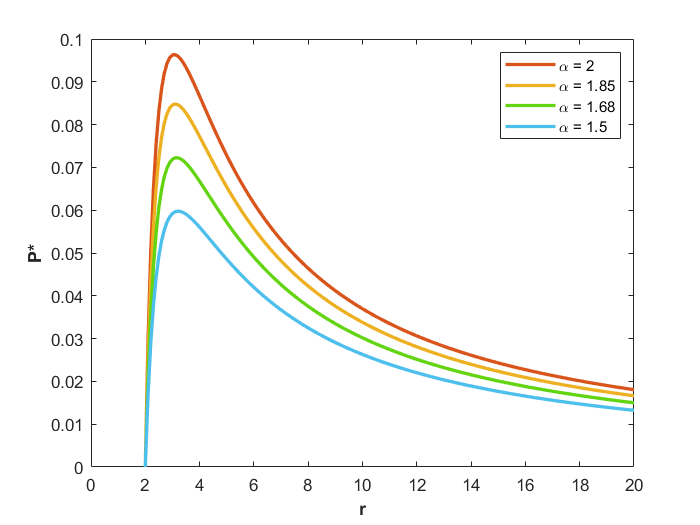
\includegraphics[width=\textwidth]{Images/FracCarnot_PvsR_a.png}
    \caption{Variasi \(\alpha\), \(\beta=0.01\).}
    \label{fig:FracCarnotPvsR_a}
  \end{subfigure}
  \hfill
  \begin{subfigure}{0.49\textwidth}
    \centering
    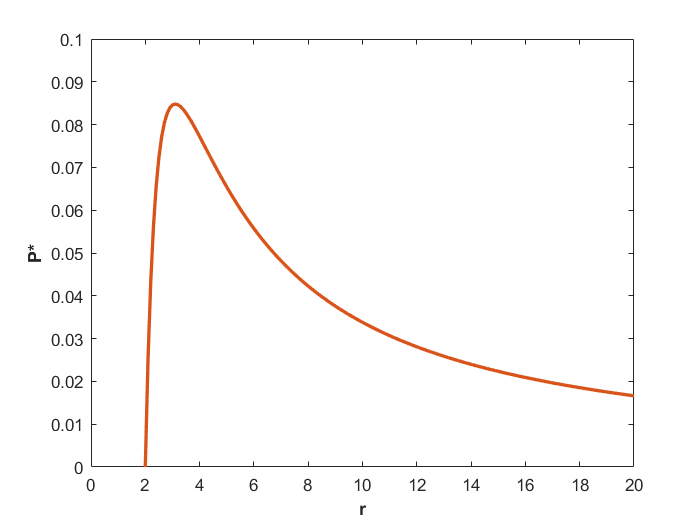
\includegraphics[width=\textwidth]{Images/FracCarnot_PvsR_B(a=1.85).png}
    \caption{Variasi \(\beta\), \(\alpha=1.85\).}
    \label{fig:FracCarnotPvsR_B}
  \end{subfigure}
  \caption{(a) \(P^*\) terhadap \(r\), divariasi terhadap \(\alpha\) dengan \(\beta\) konstan. (b) \(P^*\) terhadap \(r\), divariasi terhadap \(\beta\) dengan \(\alpha\) konstan.}
  \label{fig:FracCarnotPvsR}
\end{figure}
% \begin{figure} [H]
%     \centering
%     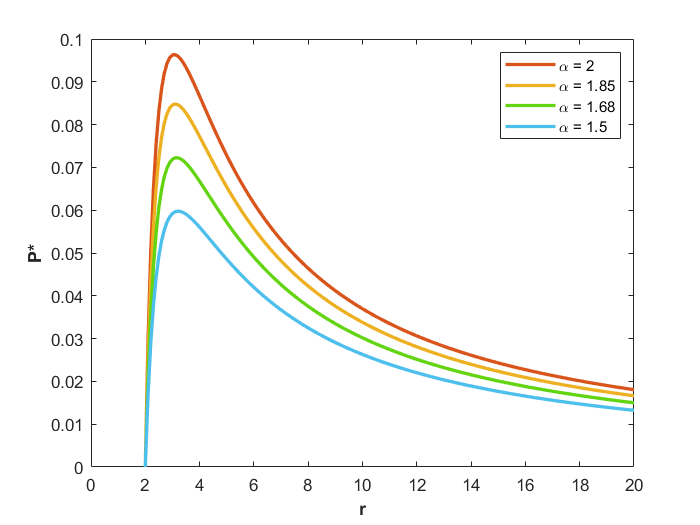
\includegraphics[width=0.6\textwidth]{Images/FracCarnot_PvsR_a.png}
%     \caption{\textit{power output} tak berdimensi \(P^*\) terhadap \(r\) pada siklus Carnot kuantum divariasi terhadap parameter fraksional \(\alpha\) dengan \(\beta = 0.01\).}
%     \label{fig:FracCarnotPvsR_a}
% \end{figure}
Diawali dengan \textit{power output} \(P^*\) terhadap parameter ekspansi \(r\). Secara umum, pola yang didapat adalah \(P^*\) meningkat secara tajam di sekitar \(r=2\) hingga sampai pada sebuah titik stasioner. Setelah melewati titik tersebut, \(P^*\) akan perlahan menurun hingga konvergensi di \(P^* = 0\) pada \(r\rightarrow\infty\). Dari grafik \ref{fig:FracCarnotPvsR_a} yang didapat, jelas bahwa parameter fraksional \(\alpha\) memiliki pengaruh terhadap \textit{power output} di mana penurunan nilai \(\alpha\) akan mengakibatkan penurunan nilai \(P^*\). Lalu pada Gambar \ref{fig:FracCarnotPvsR_B} dapat dilihat bahwa meski dikatakan divariasi terhadap \(\beta\), parameter disipasi tidak memiliki pengaruh apa pun terhadap \textit{power output} dari siklus Carnot kuantum fraksional sehingga tidak akan tampak adanya perubahan. 
\begin{figure}[H]
  \centering
  \begin{subfigure}{0.49\textwidth}
    \centering
    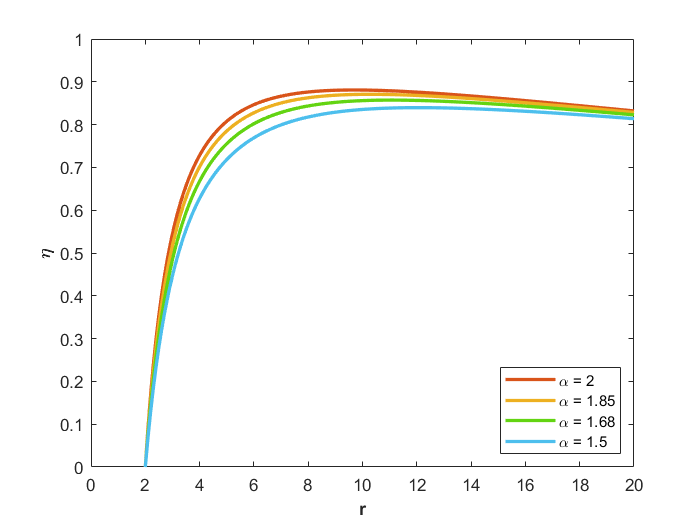
\includegraphics[width=\textwidth]{Images/FracCarnot_EtavsR_a(B=0.01).png}
    \caption{Variasi \(\alpha\), \(\beta=0.01\).}
    \label{fig:FracCarnotEtavsR_a}
  \end{subfigure}
  \hfill
  \begin{subfigure}{0.49\textwidth}
    \centering
    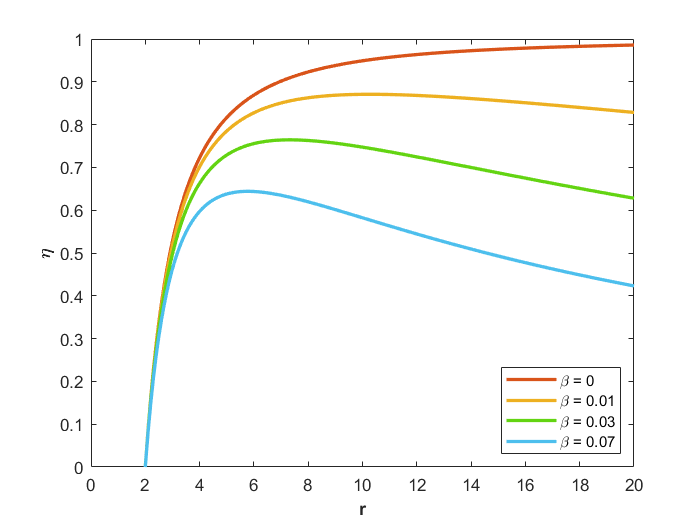
\includegraphics[width=\textwidth]{Images/FracCarnot_EtavsR_B(a=1.85).png}
    \caption{Variasi \(\beta\), \(\alpha=1.85\).}
    \label{fig:FracCarnotEtavsR_B}
  \end{subfigure}
  \caption{(a) \(\eta\) terhadap \(r\), divariasi terhadap \(\alpha\) dengan \(\beta\) konstan. (b) \(\eta\) terhadap \(r\), divariasi terhadap \(\beta\) dengan \(\alpha\) konstan.}
  \label{fig:FracCarnotEtavsR}
\end{figure}
% \begin{figure} [H]
%     \centering
%     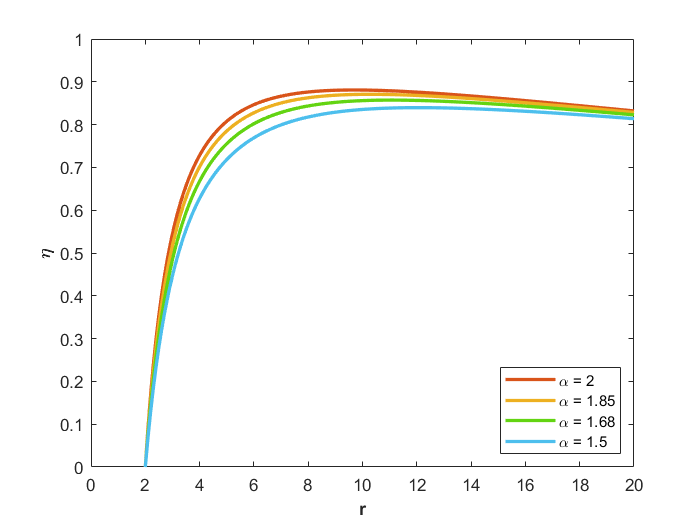
\includegraphics[width=0.6\textwidth]{Images/FracCarnot_EtavsR_a(B=0.01).png}
%     \caption{Efisiensi \(\eta\) terhadap \(r\) pada siklus Carnot kuantum divariasi terhadap parameter fraksional \(\alpha\) dengan \(\beta = 0.01\).}
%     \label{fig:FracCarnotEtavsR_a}
% \end{figure}
Dilanjutkan dengan efisiensi \(\eta\) terhadap parameter ekspansi \(r\). Pada keadaan dengan disipasi, pola yang didapat mirip seperti \(P^*\) di mana \(\eta\) meningkat secara tajam di sekitar \(r=2\) hingga sampai pada sebuah titik stasioner. Setelah melewati titik tersebut, \(\eta\) akan perlahan menurun hingga konvergensi di \(\eta = 0\) pada \(r\rightarrow\infty\). Dari grafik \ref{fig:FracCarnotEtavsR_a} yang didapat, jelas bahwa parameter fraksional \(\alpha\) memiliki pengaruh terhadap efisiensi di mana penurunan nilai \(\alpha\) akan mengakibatkan penurunan nilai \(\eta\). Namun penurunan yang diakibatkan \(\alpha\) ini tidak begitu signifikan jika dibanding dengan penurunan yang terjadi pada \(P^*\). Lalu pada Gambar \ref{fig:FracCarnotEtavsR_B} dapat dilihat bahwa pada keadaan tanpa disipasi, dimungkinkan untuk mencapai efisiensi sempurna. Namun pada keadaan tanpa disipasi, efisiensi sempurna tidak dimungkinkan lagi. Selain itu, pengaruh \(\beta\) terhadap efisiensi terlihat jauh lebih signifikan di mana kenaikan nilai \(\beta\) yang sedikit akan mengurangi efisiensi lebih banyak dibanding akibat penurunan nilai \(\alpha\).
\begin{figure}[H]
  \centering
  \begin{subfigure}{0.49\textwidth}
    \centering
    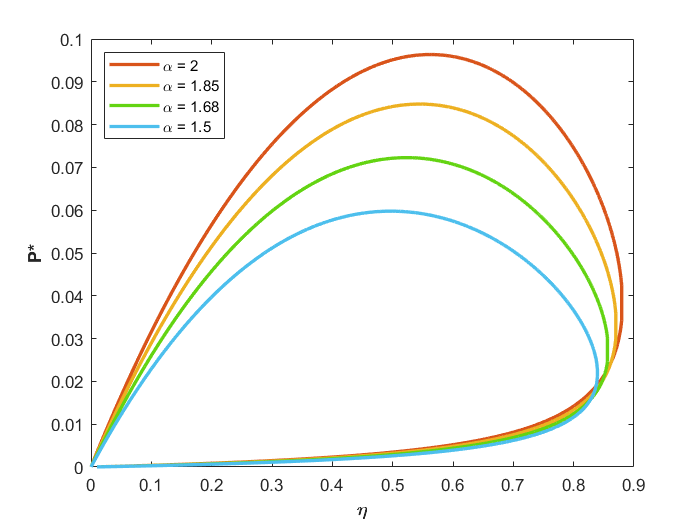
\includegraphics[width=\textwidth]{Images/FracCarnot_PvsEta_a(B=0.01).png}
    \caption{Variasi \(\alpha\), \(\beta=0.01\).}
    \label{fig:FracCarnotPvsEta_a}
  \end{subfigure}
  \hfill
  \begin{subfigure}{0.49\textwidth}
    \centering
    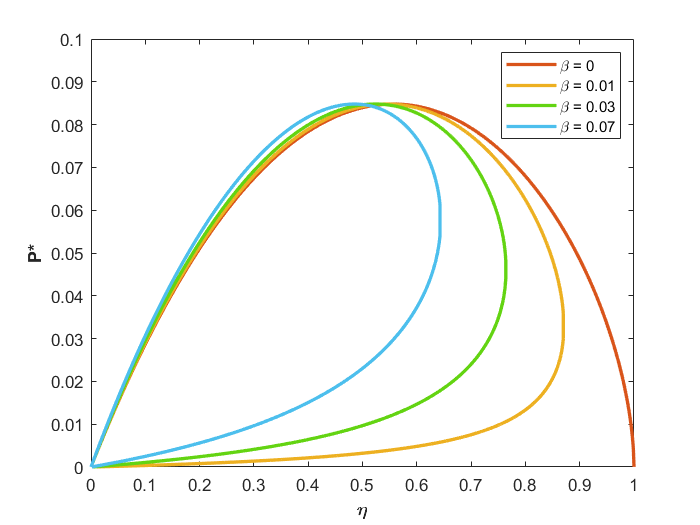
\includegraphics[width=\textwidth]{Images/FracCarnot_PvsEta_B(a=1.85).png}
    \caption{Variasi \(\beta\), \(\alpha=1.85\).}
    \label{fig:FracCarnotPvsEta_B}
  \end{subfigure}
  \caption{(a) \(P^*\) terhadap \(\eta\), divariasi terhadap \(\alpha\) dengan \(\beta\) konstan. (b) \(P^*\) terhadap \(\eta\), divariasi terhadap \(\beta\) dengan \(\alpha\) konstan.}
  \label{fig:FracCarnotPvsEta}
\end{figure}
% \begin{figure} [H]
%     \centering
%     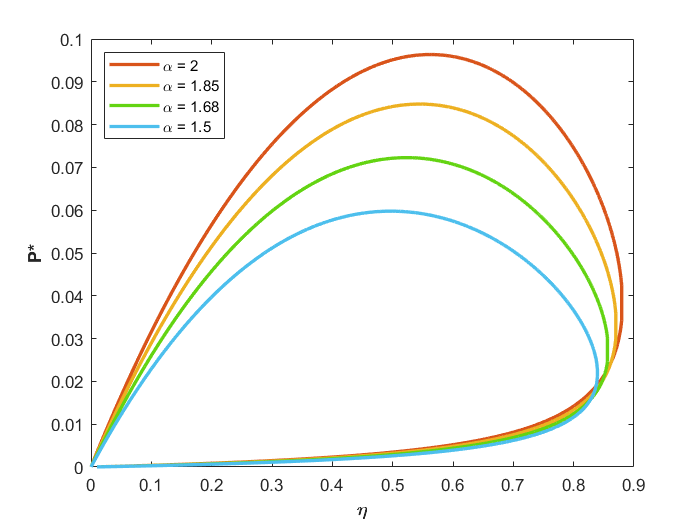
\includegraphics[width=0.6\textwidth]{Images/FracCarnot_PvsEta_a(B=0.01).png}
%     \caption{\textit{power output} tak berdimensi \(P^*\) terhadap efisiensi \(\eta\) pada siklus Carnot kuantum divariasi terhadap parameter fraksional \(\alpha\) dengan \(\beta = 0.01\).}
%     \label{fig:FracCarnotPvsEta_a}
% \end{figure}
Terakhir adalah \textit{power output} tak berdimensi \(P^*\) terhadap efisiensi \(\eta\). Pada Gambar \ref{fig:FracCarnotPvsEta_a}, keadaan yang dipilih adalah keadaan dengan disipasi sehingga tidak dimungkinkan untuk mencapai efisiensi 100\%. Cukup jelas bahwa parameter fraksional \(\alpha\) mempengaruhi \(P^*\) lebih signifikan dibanding terhadap \(\eta\). Lalu Gambar \ref{fig:FracCarnotPvsEta_B} menampilkan \(P^*\) terhadap \(\eta\) dengan variasi pada parameter disipasi \(\beta\). Seperti yang sebelumnya telah disebutkan, \(\beta\) tidak mempengaruhi \(P^*\). Karena itulah titik puncak \(P^*\) tidak berubah. Hanya saja, nampak bahwa efisiensi berubah cukup signifikan akibat perubahan nilai \(\beta\) di mana ketika disipasi diterapkan, \(\eta\) akan kembali ke 0 setelah melewati titik tertentu. Karena itulah grafik yang didapat terlihat memutar untuk nilai \(\beta>0\). Hal ini mempertegas poin yang juga sudah dijelaskan sebelumnya di mana parameter disipasi mempengaruhi efisiensi tanpa memberi pengaruh pada \textit{power output}.

% \subsection{Pengaruh Parameter Disipasi \(\beta\)}
% Setelah pengaruh parameter fraksional diketahui, di sini dilihat pengaruh parameter disipasi terhadap \textit{power output} serta efisiensi siklus. Nilai \(\alpha\) dibuat konstan. Namun untuk membedakan dengan siklus Carnot kuantum biasa, di sini nilai parameter dibuat \(\alpha=1.85\). Jadi, keadaan yang dipilih adalah keadaan dengan nilai \(\alpha\) yang lebih rendah dari 2 yang merupakan nilai \(\alpha\) untuk mesin panas kuantum biasa. Mirip seperti pada bab 2, digunakan 4 nilai \(\beta\) sebagai variasi. Di sini juga dibuat 3 grafik yaitu \(P^*\) terhadap \(r\), \(\eta\) terhadap \(r\), dan \(P^*\) terhadap \(\eta\).
% \begin{figure} [H]
%     \centering
%     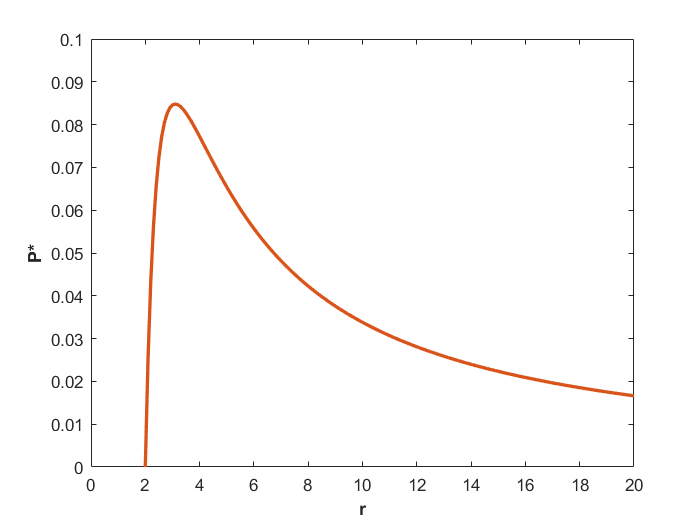
\includegraphics[width=0.6\textwidth]{Images/FracCarnot_PvsR_B(a=1.85).png}
%     \caption{\textit{power output} tak berdimensi \(P^*\) terhadap \(r\) pada siklus Carnot kuantum divariasi terhadap parameter disipasi \(\beta\) dengan \(\alpha = 1.85\).}
%     \label{fig:FracCarnotPvsR_B}
% \end{figure}
% Pertama adalah grafik \textit{power output} tak berdimensi \(P^*\) terhadap \(r\). Nampak bahwa nilai \textit{power output} yang real positif dimulai dari \(r=2\) yang mana merupakan keadaan di mana tidak terjadinya ekspansi atau kompresi isoentropis. Sehingga kerja yang dilakukan oleh siklus adalah 0. Dari sini, memperbesar \(r\) akan secara drastis meningkatkan \(P^*\) hingga mencapai titik puncak. Setelahnya, peningkatan \(r\) akan menurunkan \textit{power output}. Hal ini terjadi karena meski kerja yang dilakukan besar, waktu yang dibutuhkan untuk menyelesaikan 1 siklus menjadi besar juga dan setelah titik tertentu peningkatan kerja tidak secepat peningkatan waktu siklus. Hal ini lah yang membuat penurunan daya seiring peningkatan \(r\). Untuk parameter disipasi, perubahannya tidak mengakibatkan efek apapun terhadadp \textit{power output}. Maka dari itu, di grafik nampak tidak ada variasi dari \textit{power output} meski nilai \(\beta\) divariasi. 
% \begin{figure} [H]
%     \centering
%     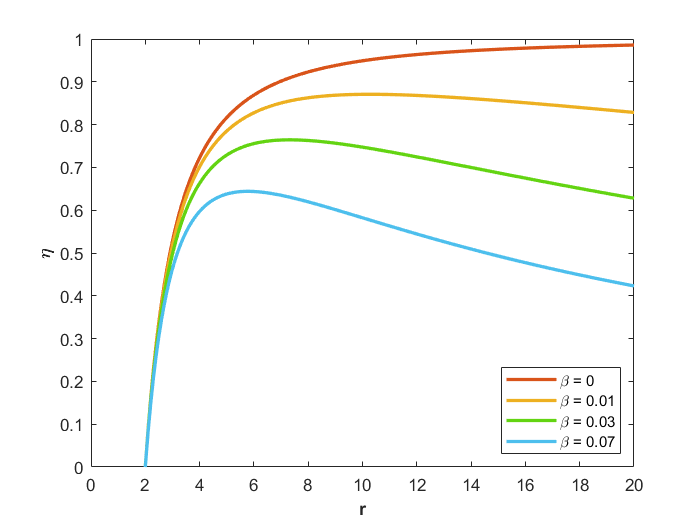
\includegraphics[width=0.6\textwidth]{Images/FracCarnot_EtavsR_B(a=1.85).png}
%     \caption{Efisiensi \(\eta\) terhadap \(r\) pada siklus Carnot kuantum divariasi terhadap parameter disipasi \(\beta\) dengan \(\alpha = 1.85\).}
%     \label{fig:FracCarnotEtavsR_B}
% \end{figure}
% Dilanjutkan dengan grafik efisiensi \(\eta\) terhadap \(r\). Seperti \textit{power output}, tampak bahwa nilai efisiensi real positif baru dimulai di \(r=2\). Penyebabnya juga sama yaitu karena di sana adalah titik tidak adanya ekspansi maupun kompresi isoentropis. Jika nilai \(r\) dinaikkan, pada keadaan tanpa disipasi nilai \(\eta\) akan tetap bisa konvergensi di \(\eta=1\). Hanya saja mengalami sedikit penurunan nilai \(\eta\) untuk nilai \(r\) yang sama. Pada keadaan dengan disipasi, akan nampak titik puncak pada efisiensi di mana terdapat titik balik dari peningkatan efisiensi. Setelah melewati titik balik ini, peningkatan nilai \(r\) akan menurunkan efisiensi. Hal ini disebabkan oleh nilai disipasi panas yang semakin meningkat seiring kenaikan \(r\). Pada \(r\rightarrow \infty\), nilai disipasi panas juga akan menjadi tak hingga. Sehingga nilai efisiensinya menjadi 0. Tentu saja seiring \(\beta\) yang semakin besar, akan menyebabkan konvergensi efisiensi ke 0 menjadi semakin cepat. 
% \begin{figure} [H]
%     \centering
%     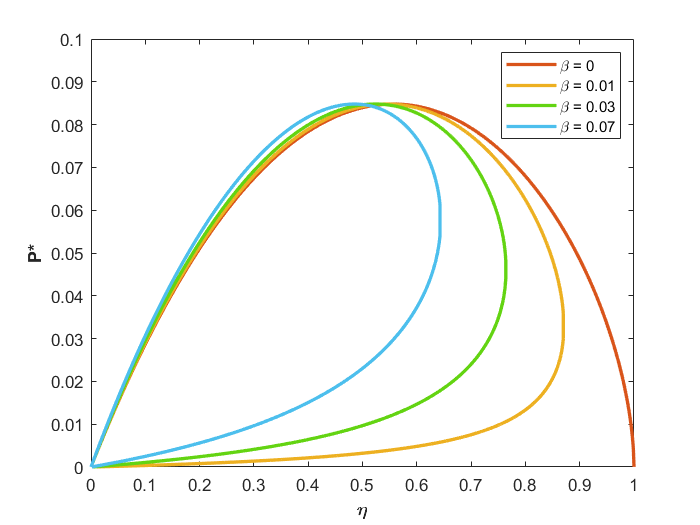
\includegraphics[width=0.6\textwidth]{Images/FracCarnot_PvsEta_B(a=1.85).png}
%     \caption{\textit{power output} tak berdimensi \(P^*\) terhadap efisiensi \(\eta\) pada siklus Carnot kuantum divariasi terhadap parameter disipasi \(\beta\) dengan \(\alpha = 1.85\).}
%     \label{fig:FracCarnotPvsEta_B}
% \end{figure}
% Terakhir adalah grafik \textit{power output} tak berdimensi \(P^*\) terhadap efisiensi \(\eta\) yang mempertegas poin yang telah disampaikan pada 2 grafik sebelumnya. Pada keadaan tanpa disipasi, dimungkinkan untuk mencapai efisiensi sempurna. Hanya saja \textit{power output}nya 0 karena waktu siklusnya terlalu lama. Perbedaan nilai \(\alpha\) yang digunakan pada grafik ini menyebabkan penurunan nilai puncak dari dari \(P^*\) namun pergeserannya tidak begitu terlihat. Pada keadaan dengan disipasi, baik efisiensi maupun \textit{power output} akan bernilai 0 pada \(r=2\) dan \(r\rightarrow \infty\). Hal ini nampak pada grafik yang dimulai dari 0 lalu memutar kembali ke arah 0 setelah melewati titik tertentu. Perbedaan nilai \(\beta\) menyebabkan perbedaan titik baliknya. Di mana nilai \(\beta\) yang lebih kecil memungkinkan efisiensi untuk mencapai nilai yang lebih tinggi. Otomatis berlaku sebaliknya juga di mana semakin tinggi nilai \(\beta\) akan semakin rendah nilai maksimum efisiensi yang dimungkinkan.

\section{Siklus Otto Kuantum Fraksional}
Siklus selanjutnya adalah siklus Otto kuantum fraksional. Secara umum \textit{setup}-nya sama seperti siklus Otto kuantum biasa. Gambaran dari proses yang terjadi diilustraikan oleh Gambar \ref{fig:QOttoCycle} yang ditampilkan pada bab 2. Siklus ini dibuka dengan masuknya panas melalui proses isovolume pada segmen \(AB\). Di sini, panas masuk tanpa mengubah lebar sumur atau bisa dikatakan \(L_A=L_B\). Karena lebar sumur tidak berubah, tidak ada kerja yang dilakukan selama proses ini. Sehingga besaran panas yang masuk hanya mempengaruhi perubahan energi dalamnya saja.
\begin{align}
    Q_{AB} = \Delta U_{AB} + \dot{Q_r}\tau
    % &= E_2(L_B) - E_1(L_A) + \dot{Q_r}\tau \\
    % &= E_2(L_A) - E_1(L_A) + \dot{Q_r}\tau \\
    % &= D_\alpha\left(\frac{2\hbar\pi}{L_A}\right)^\alpha - D_\alpha\left(\frac{\hbar\pi}{L_A}\right)^\alpha + \dot{Q_r}\tau \\
    % &= D_\alpha\left(\frac{\hbar\pi}{L_A}\right)^\alpha (2^\alpha - 1) + \dot{Q_r}\tau
\end{align}
Bentuk persamaan rerata energinya mirip seperti siklus Carnot. Dengan demikian, didapat \(Q_{AB}\) sebagai berikut:
\begin{align}
    Q_{AB} = E_2(L_B) - E_1(L_A) + \dot{Q_r}\tau = D_\alpha\left(\frac{\hbar\pi}{L_A}\right)^\alpha (2^\alpha - 1) + \dot{Q_r}\tau \label{eq:FracOttoQab}
\end{align}
Proses dilanjutkan dengan proses isoentropis pada segmen \(BC\). Di sini tidak terjadi pertukaran panas. Sumur mengalami ekspansi dari \(L_B\) ke \(L_C\), namun tidak mengubah tingkatan energi eigennya. Dilanjutkan dengan pembuangan panas melalui proses isovolume pada segmen \(CD\). Sama seperti saat panas masuk, tidak ada perubahan panjang sumur pada proses ini (\(L_C = L_D\)). Sehingga besaran panas yang masuk dapat diketahui sebagai berikut:
\begin{align}
    Q_{CD} = |\Delta U| + \dot{Q_r}\tau = D_\alpha\left(\frac{\hbar\pi}{L_C}\right)^\alpha (2^\alpha - 1) + \dot{Q_r}\tau \label{eq:FracOttoQcd}
    % &= \left| E_1(L_D) - E_2(L_C) \right| + \dot{Q_r}\tau \\
    % &= E_2(L_C) - E_1(L_C) + \dot{Q_r}\tau \\
\end{align}
Siklus ditutup pada segmen \(DA\) di mana terjadi proses kompresi isoentropis. Dengan begitu, dapat diketahui kerja yang dilakukan selama satu siklus menggunakan persamaan (\ref{eq:FracOttoQab}) dan (\ref{eq:FracOttoQcd}).
\begin{align}
    W = Q_{AB} - Q_{CD} = D_\alpha(\hbar\pi)^\alpha (2^\alpha - 1)\left(\frac{1}{L_A^\alpha} - \frac{1}{L_C^\alpha}\right) \label{eq:FracOttoW}
\end{align}
\par Setelah didapatkan besaran kalor yang masuk dan keluar serta kerja siklus, \textit{power output} serta efisiensi siklus bisa didapatkan. Pertama adalah \textit{power output} yang didapatkan menggunakan persamaan (\ref{eq:TauDef}) dan (\ref{eq:FracOttoQcd}) sebagai berikut:
\begin{align}
    P = \frac{W}{\tau} = \frac{D_\alpha(\hbar\pi)^\alpha(2^\alpha - 1)\overline{\nu}}{2L_A^{\alpha+1}} \left( \frac{r^\alpha - 1}{r^{\alpha+1} - r^\alpha}\right) 
    % &= \frac{D_\alpha(\hbar\pi)^\alpha(2^\alpha - 1)\overline{\nu}}{2(L_C - L_A)} \left( \frac{1}{L_A^\alpha} - \frac{1}{L_C^\alpha}\right) \\
    % &= \frac{D_\alpha(\hbar\pi)^\alpha(2^\alpha - 1)\overline{\nu}}{2(L_C - L_A)} \left( \frac{\frac{L_C^\alpha}{L_A^\alpha} - 1}{L_C^\alpha}\right) \\
\end{align}
Jika mempertimbangkan bentuk \textit{power output} tak berdimensi siklus Otto kuantum biasa, maka \textit{power output} tak berdimensi siklus fraksionalnya bisa didapat sebaagai berikut:
\begin{align}
    P^* = \frac{2^\alpha - 1}{4}\left(\frac{r^\alpha - 1}{r^{\alpha+1} - r^\alpha}\right)
\end{align}
Dengan \(A=2D_\alpha(\hbar\pi)^\alpha\overline{\nu}/L_A^{\alpha+1}\). Kemudian efisiensi dari siklus ini didapatkan menggunakan persamaan (\ref{eq:FracOttoQab}) dan (\ref{eq:FracOttoW}),
\begin{align}
    \eta = \frac{W}{Q_{AB}} = \frac{D_\alpha(\hbar\pi)^\alpha (2^\alpha - 1)\left(\frac{1}{L_A^\alpha} - \frac{1}{L_C^\alpha}\right)}{D_\alpha\left(\frac{\hbar\pi}{L_A}\right)^\alpha (2^\alpha - 1) + \frac{2\dot{Q_r}(L_C-L_A)}{\overline{\nu}}}
\end{align}
Untuk menyederhanakan perhitungan dan menghilangkan dimensi efisiensi, diasumsikan disipasi panas memiliki bentuk sebagai berikut:
\begin{align}
    \dot{Q_r} = \beta \frac{D_\alpha\overline{\nu}}{2L_A}\left(\frac{\hbar\pi}{L_A}\right)^\alpha (2^\alpha - 1)
\end{align}
Dengan begitu, didapat bentuk efisiensi
\begin{align}
    % \eta &= \frac{D_\alpha(\hbar\pi)^\alpha (2^\alpha - 1)\left(\frac{1}{L_A^\alpha} - \frac{1}{L_C^\alpha}\right)}{D_\alpha\left(\frac{\hbar\pi}{L_A}\right)^\alpha (2^\alpha - 1) + \beta \frac{D_\alpha\overline{\nu}}{2L_A}\left(\frac{\hbar\pi}{L_A}\right)^\alpha (2^\alpha - 1)\cdot\frac{2(L_C-L_A)}{\overline{\nu}}} \\
    % &= \frac{L_A^\alpha\left(\frac{1}{L_A^\alpha} - \frac{1}{L_C^\alpha}\right)}{1 + \beta \frac{(L_C-L_A)}{L_A}} \\
    \eta = \frac{1 - \left(\frac{1}{r}\right)^\alpha}{1+\beta(r-1)}
\end{align}
Di sini, nilai efisiensi real positif dimulai dari \(r=1\) dengan \(\eta=0\). Namun uniknya, nilai \textit{power output} tidak 0 saat \(r\rightarrow 1\). Pada keadaan dengan nilai \(\alpha=2\), nilai \(P^*\rightarrow 1.5\) pada \(r\rightarrow 1\). Sedangkan jika nilai \(\alpha\) lebih kecil, akan didapatkan nilai \(P^*\) yang lebih kecil pula pada keadaan yang sama.
\par Seperti siklus sebelumnya, tinjauan akan pengaruh dari parameter fraksional \(\alpha\) dan disipasi \(\beta\) dipisah. Di sini, dibuat 3 grafik untuk variasi \(\alpha\) dan 3 juga untuk variasi \(\beta\). Masing-masing grafik tersebut adalah; \(P^*\) terhadap \(r\), \(\eta\) terhadap \(r\), dan \(P^*\) terhadap \(eta\). Saat \(\alpha\) divariasi, parameter disipasi dibuat konstan dengan nilai \(\beta=0.01\) sehingga tinjauan ada pada keadaan dengan disipasi. Saat \(\beta\) divariasi, parameter \(\alpha\) dibuat konstan dengan nilai \(\alpha=1.85\) sehingga tinjauan ada pada keadaan fraksional.
\begin{figure}[H]
  \centering
  \begin{subfigure}{0.49\textwidth}
    \centering
    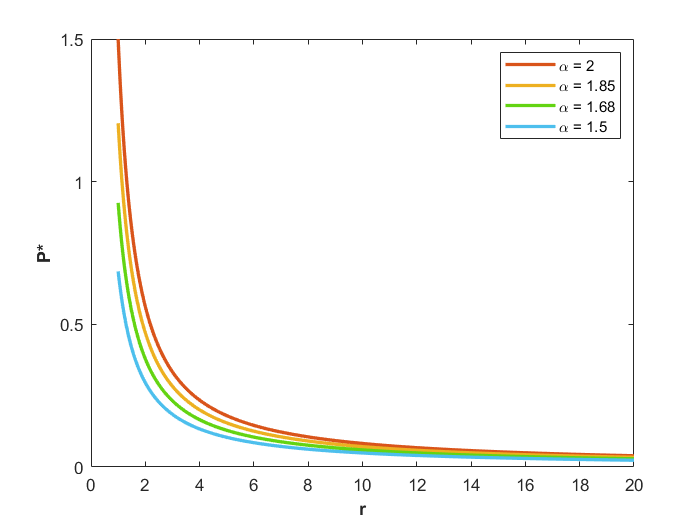
\includegraphics[width=\textwidth]{Images/FracOtto_PvsR_a(B=0.01).png}
    \caption{Variasi \(\alpha\), \(\beta=0.01\).}
    \label{fig:FracOttoPvsR_a}
  \end{subfigure}
  \hfill
  \begin{subfigure}{0.49\textwidth}
    \centering
    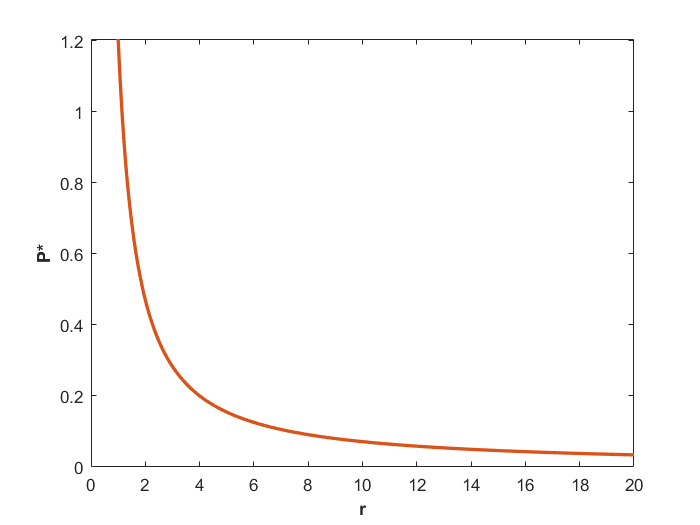
\includegraphics[width=\textwidth]{Images/FracOtto_PvsR_B(a=1.85).png}
    \caption{Variasi \(\beta\), \(\alpha=1.85\).}
    \label{fig:FracOttoPvsR_B}
  \end{subfigure}
  \caption{(a) \(P^*\) terhadap \(r\), divariasi terhadap \(\alpha\) dengan \(\beta\) konstan. (b) \(P^*\) terhadap \(r\), divariasi terhadap \(\beta\) dengan \(\alpha\) konstan.}
  \label{fig:FracOttoPvsR}
\end{figure}
% \begin{figure} [H]
%     \centering
%     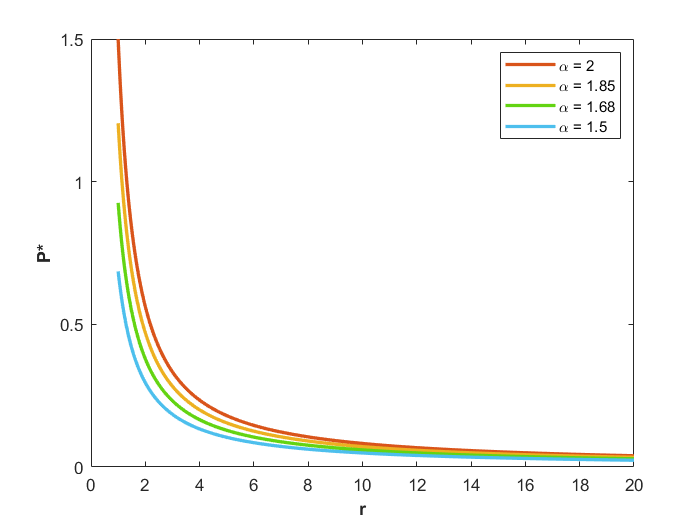
\includegraphics[width=0.6\textwidth]{Images/FracOtto_PvsR_a(B=0.01).png}
%     \caption{\textit{power output} tak berdimensi \(P^*\) terhadap \(r\) pada siklus Otto kuantum divariasi terhadap parameter fraksional \(\alpha\) dengan \(\beta = 0.01\).}
%     \label{fig:FracOttoPvsR_a}
% \end{figure}
Diawali dengan \textit{power output} \(P^*\) terhadap parameter ekspansi \(r\). Secara umum, pola yang didapat adalah \(P^*\) memiliki nilai terbesar di \(r=1\). Lalu dengan naiknya nilai \(r\), \(P^*\) akan turun hingga konvergensi di \(P^*\rightarrow0\) pada \(r\rightarrow\infty\). Daya yang meemiliki nilai di \(r=1\) ini diakibatkan oleh kecilnya daya dari grafik \ref{fig:FracOttoPvsR_a} dikompensasi oleh kecilnya waktu yang diperlukan untuk menyelesaikan 1 siklus. Lalu, jelas bahwa parameter fraksional \(\alpha\) memiliki pengaruh terhadap \textit{power output} di mana penurunan nilai \(\alpha\) akan mengakibatkan penurunan nilai \(P^*\). Lalu pada Gambar \ref{fig:FracOttoPvsR_B} dapat dilihat bahwa meski dikatakan divariasi terhadap \(\beta\), parameter disipasi tidak memiliki pengaruh apa pun terhadap \textit{power output} dari siklus Otto kuantum fraksional sehingga tidak akan tampak adanya perubahan. 
% Pertama adalah \textit{power output} terhadap \(P^*\) terhadap \(r\). Pola yang didapat adalah nilai \textit{power output} tinggi di awal dan menurun seiring naiknya \(r\). Di sini sebetulnya nilai \(P^*\) masih memiliki nilai real positif di \(r<1\). Hanya saja, jika keadaan tersebut dibiarkan, akan didapat nilai negatif yang mana tidak fisis. Maka dari itu, di sini grafik untuk \(r<1\) tidak dimasukkan pada gambar yang ditampilkan. Untuk pengaruh parameter fraksional, tampak bahwa penurunan nilai \(\alpha\) berakibat pana penurunan \textit{power output} secara cukup signifikan terutama untuk nilai \(r\) yang kecil. Sedangkan Untuk nilai \(r\) yang besar, perubahannya tidak terlalu besar.
\begin{figure}[H]
  \centering
  \begin{subfigure}{0.49\textwidth}
    \centering
    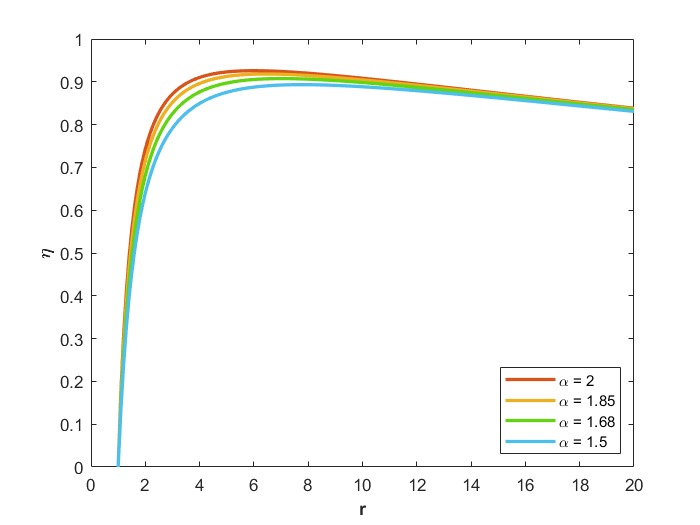
\includegraphics[width=\textwidth]{Images/FracOtto_EtavsR_a(B=0.01).png}
    \caption{Variasi \(\alpha\), \(\beta=0.01\).}
    \label{fig:FracOttoEtavsR_a}
  \end{subfigure}
  \hfill
  \begin{subfigure}{0.49\textwidth}
    \centering
    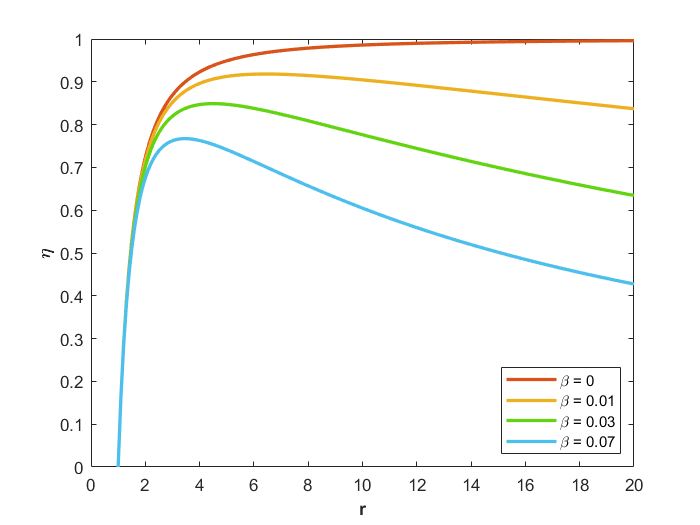
\includegraphics[width=\textwidth]{Images/FracOtto_EtavsR_B(a=1.85).png}
    \caption{Variasi \(\beta\), \(\alpha=1.85\).}
    \label{fig:FracOttoEtavsR_B}
  \end{subfigure}
  \caption{(a) \(\eta\) terhadap \(r\), divariasi terhadap \(\alpha\) dengan \(\beta\) konstan. (b) \(\eta\) terhadap \(r\), divariasi terhadap \(\beta\) dengan \(\alpha\) konstan.}
  \label{fig:FracOttoEtavsR}
\end{figure}
Kedua adalah efisiensi \(\eta\) terhadap parameter ekspansi \(r\). Pada keadaan dengan disipasi, pola yang didapat adalah \(\eta\) meningkat secara tajam di sekitar \(r=1\) hingga sampai pada sebuah titik stasioner. Setelah melewati titik tersebut, \(\eta\) akan perlahan menurun hingga konvergensi di \(\eta \rightarrow 0\) pada \(r\rightarrow\infty\). Dari grafik \ref{fig:FracOttoEtavsR_a} yang didapat, jelas bahwa parameter fraksional \(\alpha\) memiliki pengaruh terhadap efsiensi di mana penurunan nilai \(\alpha\) akan mengakibatkan penurunan nilai \(\eta\). Namun penurunan yang diakibatkan \(\alpha\) ini tidak begitu signifikan jika dibanding dengan penurunan yang terjadi pada \(P^*\). Lalu pada Gambar \ref{fig:FracOttoEtavsR_B} dapat dilihat bahwa pada keadaan tanpa disipasi, dimungkinkan untuk mencapai efisiensi sempurna. Namun pada keadaan tanpa disipasi, efisiensi sempurna tidak dimungkinkan terjadi. Selain itu, pengaruh \(\beta\) terhadap efisiensi terlihat jauh lebih signifikan di mana kenaikan nilai \(\beta\) akan mengurangi efisiensi lebih besar dibanding akibat penurunan nilai \(\alpha\).
% \begin{figure} [H]
%     \centering
%     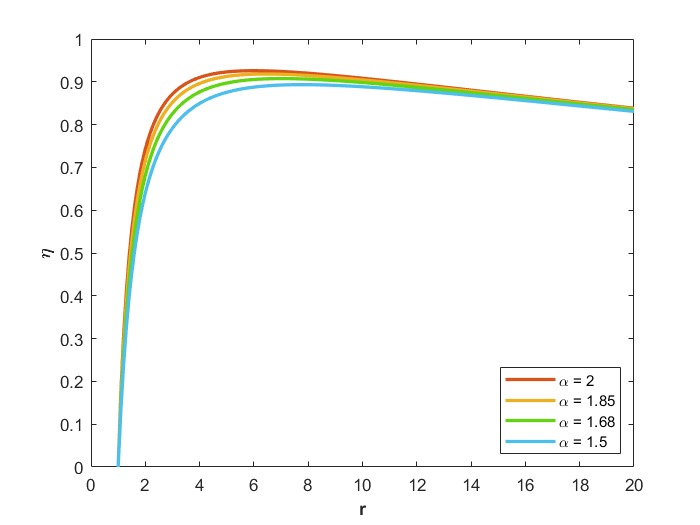
\includegraphics[width=0.6\textwidth]{Images/FracOtto_EtavsR_a(B=0.01).png}
%     \caption{Efisiensi \(\eta\) terhadap \(r\) pada siklus Otto kuantum divariasi terhadap parameter fraksional \(\alpha\) dengan \(\beta = 0.01\).}
%     \label{fig:FracOttoEtavsR_a}
% \end{figure}
% Selanjutnya adalah efisiensi \(\eta\) terhadap \(r\). Karena keadaan yang digunakan adalah keadaan dengan dispasi, didapatkan pola di mana \(\eta\) akan meningkat seiring kenaikan \(r\) hingga mencapai titik tertentu. Lalu kemudian turun seiring kenaikan \(r\) hingga mencapai \(\eta\rightarrow 0\) di \(r\rightarrow \infty\). Grafik ini juga memperjelas pernyataan mengenai grafik sebelumnya di mana nilai \(\eta\) baru bernilai real positif di \(r=1\). Lalu untuk efek parameter fraksional, nampak bahwa pengaruhnya tidak terlalu besar jika dibanding pengaruh terhadap \textit{power output}.
\begin{figure}[H]
  \centering
  \begin{subfigure}{0.49\textwidth}
    \centering
    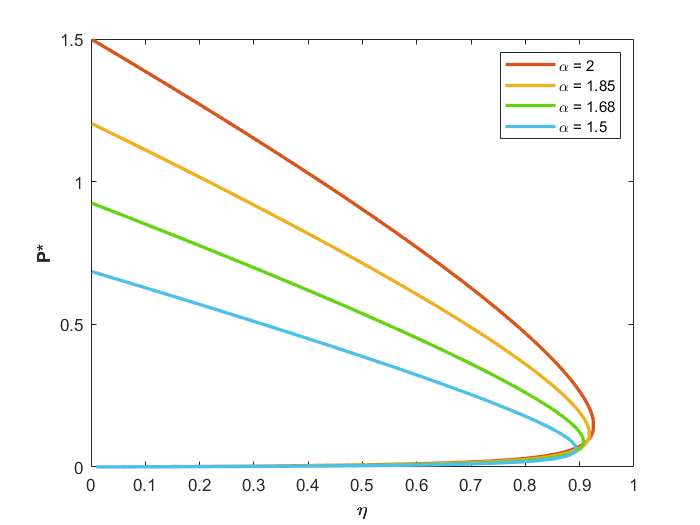
\includegraphics[width=\textwidth]{Images/FracOtto_PvsEta_a(B=0.01).png}
    \caption{Variasi \(\alpha\), \(\beta=0.01\).}
    \label{fig:FracOttoPvsEta_a}
  \end{subfigure}
  \hfill
  \begin{subfigure}{0.49\textwidth}
    \centering
    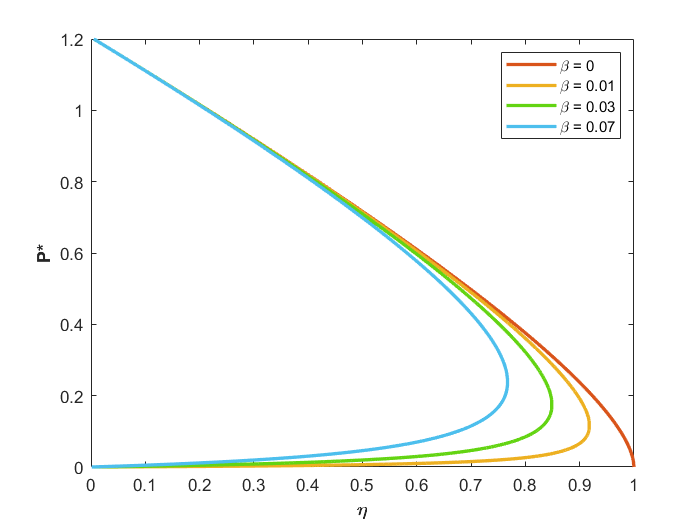
\includegraphics[width=\textwidth]{Images/FracOtto_PvsEta_B(a=1.85).png}
    \caption{Variasi \(\beta\), \(\alpha=1.85\).}
    \label{fig:FracOttoPvsEta_B}
  \end{subfigure}
  \caption{(a) \(P^*\) terhadap \(\eta\), divariasi terhadap \(\alpha\) dengan \(\beta\) konstan. (b) \(P^*\) terhadap \(\eta\), divariasi terhadap \(\beta\) dengan \(\alpha\) konstan.}
  \label{fig:FracOttoPvsEta}
\end{figure}
% \begin{figure} [H]
%     \centering
%     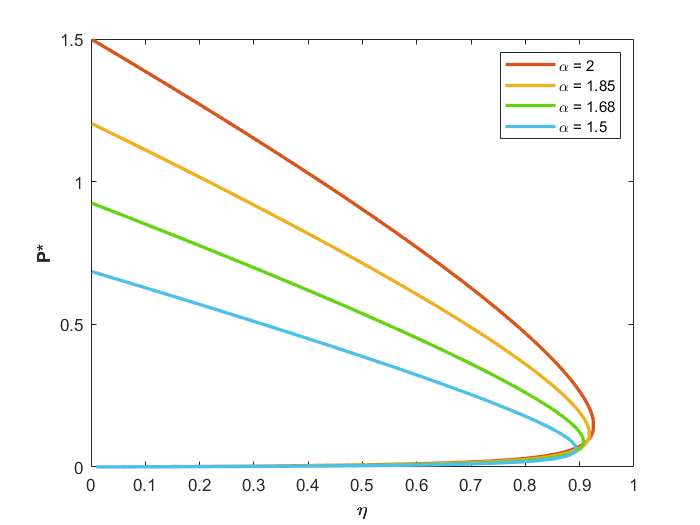
\includegraphics[width=0.6\textwidth]{Images/FracOtto_PvsEta_a(B=0.01).png}
%     \caption{\textit{power output} tak berdimensi \(P^*\) terhadap efisiensi \(\eta\) pada siklus Otto kuantum divariasi terhadap parameter fraksional \(\alpha\) dengan \(\beta = 0.01\).}
%     \label{fig:FracOttoPvsEta_a}
% \end{figure}
Terakhir adalah \textit{power output} tak berdimensi \(P^*\) terhadap efisiensi \(\eta\). Pola yang didapat berbeda dibanding siklus lainnya di mana \(P^*\) tidak dimulai dari 0 melainkan dari nilai tertentu bergantung pada nilai \(\alpha\) yang digunakan. Pada Gambar \ref{fig:FracOttoPvsEta_a}, keadaan yang dipilih adalah keadaan dengan disipasi sehingga tidak dimungkinkan untuk mencapai efisiensi 100\%. Cukup jelas bahwa parameter fraksional \(\alpha\) mempengaruhi \(P^*\) lebih signifikan dibanding terhadap \(\eta\) di mana penurunan nilai mula-mula \(P^*\) lebih besar dari pergeseran nilai puncak \(\eta\) yang terjadi. Lalu Gambar \ref{fig:FracOttoPvsEta_B} menampilkan \(P^*\) terhadap \(\eta\) dengan variasi pada parameter disipasi \(\beta\). Seperti yang sebelumnya telah disebutkan, \(\beta\) tidak mempengaruhi \(P^*\). Karena itulah titik puncak \(P^*\) tidak berubah. Hanya saja, nampak bahwa efisiensi berubah cukup signifikan akibat perubahan nilai \(\beta\) di mana ketika disipasi diterapkan, \(\eta\) akan kembali ke 0 setelah melewati titik tertentu. Karena itulah grafik yang didapat terlihat memutar untuk nilai \(\beta>0\). Hal ini mempertegas poin yang juga sudah dijelaskan sebelumnya di mana parameter disipasi mempengaruhi efisiensi tanpa memberi pengaruh pada \textit{power output}.

\section{Siklus Brayton Kuantum Fraksional}
Siklus terakhir adalah siklus Brayton kuantum fraksional.\textit{Setup} yang digunakan sama seperti siklus Brayton kuantum biasa. Gambaran dari proses yang terjadi dapat dilihat pada Gambar \ref{fig:QBraytonCycle} yang tertera pada Bab 2. Siklus ini dibuka pada segmen \(AB\) dengan masuknya panas melalui proses isobarik atau bisa ditulis \(F_{AB}(L) = F(L_A) = F(L_B)\) yang memiliki bentuk eksplisit sebagai berikut:
\begin{align}
    F_{AB}(L) = \alpha D_\alpha\frac{(\hbar\pi)^\alpha}{L_A^{\alpha+1}} = \alpha D_\alpha\frac{(2\hbar\pi)^\alpha}{L_B^{\alpha+1}} \label{eq:FracBraytonConstF}
\end{align}
Perubahan lebar sumur dapat diketahui melalui persamaan (\ref{eq:FracBraytonConstF}) ini, di mana didapatkan,
\begin{align}
    L_B = 2^\frac{\alpha}{\alpha+1}L_A \label{eq:FracBraytonLaLbRelation}
\end{align}
Siklus ini cukup unik karena dibanding 2 siklus fraksional sebelumnya, di sini perubahan lebar sumur saat panas masuk dapat dipengaruhi oleh parameter fraksional, sementara sebelumnya tidak. Kerja yang dilakukan selama proses masuknya panas ini dapat diketahui sebagai berikut:
\begin{align}
    W_{AB} &= \int_{L_A}^{L_B} F_{AB} dL \\
    % W_{AB} &= \alpha D_\alpha\frac{(\hbar\pi)^\alpha}{L_A^{\alpha+1}} (L_B - L_A)
\end{align}
Dengan melakukan substitusi persamaan (\ref{eq:FracBraytonConstF}) dan menggunakan hubungan lebar sumur pada persamaan (\ref{eq:FracBraytonLaLbRelation}), \(W_{AB}\) dapat dinyatakan sebagai berikut: 
\begin{align}
    W_{AB} = \alpha D_\alpha\left(\frac{\hbar\pi}{L_A}\right)^\alpha (2^\frac{\alpha}{\alpha+1}-1)
\end{align}
Perubahan energi dalam yang terjadi dapat didapatkan sebagai berikut:
\begin{align}
    \Delta U_{AB} = E_2(L_B) - E_1(L_A) = D_\alpha(\hbar\pi)^\alpha \left(\frac{2^\alpha}{L_B^\alpha} - \frac{1}{L_A^\alpha}\right)
\end{align}
Besaran \(\Delta U_{AB}\) juga dapat dinyatakan sebagai fungsi \(L_A\) saja.
\begin{align}
    \Delta U_{AB} = D_\alpha \left(\frac{\hbar\pi}{L_A}\right)^\alpha (2^\frac{\alpha}{\alpha+1} - 1)
\end{align}
Panas yang masuk ke siklus \(Q_{AB}\) dapat diketahui melalui kuantitas kerja serta perubahan energi dalam yang telah dinyatakan sebelumnya. 
\begin{align}
    Q_{AB} &= W_{AB} + \Delta U_{AB} + \dot{Q_r}\tau \notag \\
    &= D_\alpha\left(\frac{\hbar\pi}{L_A}\right)^\alpha (\alpha+1)(2^\frac{\alpha}{\alpha+1}-1) + \dot{Q_r}\tau \label{eq:FracBraytonQab}
\end{align}
Siklus dilanjutkan dengan ekspansi isoentropis pada segmen \(BC\). Di sini, tembok bergerak dari \(L_B\) menuju \(L_C\) tanpa mengubah tingkatan energi eignnya. 
\par Kemudian, siklus berlanjut pada segmen \(CD\) di mana terjadi pembuangan panas melalui proses isobarik. Tentunya gaya pada proses ini konstan atau dapat ditulis \(F_{CD}(L) = F(L_C) = F_(L_D)\) yang mengarah pada hubungan lebar sumur \(L_D = 2^{-\frac{\alpha}{\alpha+1}} L_C\). Hubungan ini selanjutnya mengarahkan kepada besaran kerja serta perubahan energi dalam yang terjadi pada segmen \(CD\). Keduanya dapat dinyatakan sebagai berikut:
\begin{align}
    W_{CD} &= - \frac{\alpha D_\alpha}{2^\frac{\alpha}{\alpha+1}} \left(\frac{2\hbar\pi}{L_C}\right)^\alpha (2^\frac{\alpha}{\alpha+1}-1) \\
    \Delta U_{CD} &= -\frac{D_\alpha}{2^\frac{\alpha}{\alpha+1}} \left(\frac{2\hbar\pi}{L_C}\right)^\alpha (2^\frac{\alpha}{\alpha+1}-1)
\end{align}
Dengan begitu, besaran panas yang keluar dari siklus pada proses ini dapat diketahui. 
\begin{align}
    Q_{CD} &= |W_{CD}| + |\Delta U_{CD}| + \dot{Q_r}\tau \notag \\
    &= \frac{D_\alpha}{2^\frac{\alpha}{\alpha+1}} \left(\frac{2\hbar\pi}{L_C}\right)^\alpha (\alpha+1)(2^\frac{\alpha}{\alpha+1}-1) + \dot{Q_r}\tau \label{eq:FracBraytonQcd}
\end{align}
Siklus kemudian diakhiri pada segmen \(DA\) dengan proses kompresi isoentropis. Di sini, tembok bergerak dari \(L_D\) menuju \(L_A\) tanpa mengubah tingkatan energi eigennya. 
\par Kerja yang dilakukan oleh siklus dapat diperoleh menggunakan kuantitas \(Q_{AB}\) dan \(Q_{CD}\) pada persamaan (\ref{eq:FracBraytonQab}) dan (\ref{eq:FracBraytonQcd}). Secara eksplisit, kerja yang dilakukan oleh siklus Brayton kuantum fraksional ini dapat dinyatakan sebagai berikut:
\begin{align}
    W &= Q_{AB} - Q_{CD} \notag \\
    &= D_\alpha(\hbar\pi)^\alpha (\alpha+1)(2^\frac{\alpha}{\alpha+1}-1) \left(\frac{1}{L_A^\alpha} - \frac{2^\frac{\alpha^2}{\alpha+1}}{L_C^\alpha}\right) \label{eq:FracBraytonW}
\end{align}
Dengan begitu, \textit{power output} serta efisiensi bisa diperoleh menggunakan kuantitas panas yang masuk \(Q_{AB}\) pada persamaan (\ref{eq:FracBraytonQab}) dan juga kerja \(W\) pada persamaan (\ref{eq:FracBraytonW}). Pertama adalah \textit{power output} yang jika dibuat sebagai fungsi parameter ekspansi \(r\) akan memiliki bentuk sebagai berikut:
\begin{align}
    P = \frac{W}{\tau} = \frac{D_\alpha (\hbar\pi)^\alpha \overline{\nu}}{2L_A^{\alpha+1}} (\alpha+1)(2^\frac{\alpha}{\alpha+1}-1) \left(\frac{r^\alpha-2^\frac{\alpha^2}{\alpha+1}}{r^{\alpha+1}-r^\alpha}\right)
\end{align}
Sehingga, \textit{power output} tak berdimensinya adalah
\begin{align}
    P^* = \frac{W}{A\tau} = \frac{\alpha+1}{4}(2^\frac{\alpha}{\alpha+1}-1) \left(\frac{r^\alpha-2^\frac{\alpha^2}{\alpha+1}}{r^{\alpha+1}-r^\alpha}\right)
\end{align}
Dengan \(A=2D_\alpha(\hbar\pi)^\alpha\overline{\nu}/L_A^{\alpha+1}\). Berikutnya, jika diasumsikan disipasi panas memiliki bentuk sebagai berikut:
\begin{align}
    \dot{Q_r} = \beta \frac{D_\alpha \overline{\nu}}{2L_A} \left(\frac{\hbar\pi}{L_A}\right)^\alpha (\alpha+1)(2^\frac{\alpha}{\alpha+1}-1)
\end{align}
Maka akan didapat bentuk efisiensi,
\begin{align}
    \eta = \frac{W}{Q_{AB}} = \frac{1 - \left(\frac{2^\frac{\alpha}{\alpha+1}}{r} \right)^\alpha}{1 + \beta(r-1)}
\end{align}
Dapat dilihat bahwa titik di mana nilai efisiensi menjadi real positif dapat berubah oleh parameter fraksional \(\alpha\) yang mana pada kedua siklus sebelumnya tidak bisa. Dari nilai \textit{power output} serta efisiensi yang didapat, pengaruh dari setiap parameter yang terlibat bisa ditinjau. Untuk itu, dibuat 3 jenis grafik: \(P^*\) terhadap \(r\), \(\eta\) terhadap \(r\), dan \(P^*\) terhadap \(\eta\). Tiap jenis grafik tersebut akan terbagi 2, divariasi terhadap \(\alpha\) dan terhadap \(\beta\). Untuk variasi terhadap \(\alpha\), \(\beta\) dibuat konstan dengan nilai 0.01. Sedangkan saat dilakukan variasi terhadap \(\beta\), \(\alpha\) dibuat konstan dengan nilai 1.85.
\begin{figure}[H]
  \centering
  \begin{subfigure}{0.49\textwidth}
    \centering
    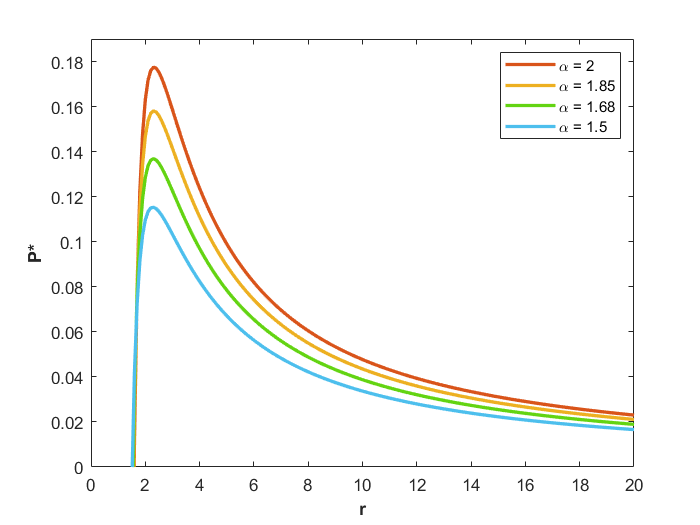
\includegraphics[width=\textwidth]{Images/FracBrayton_PvsR_a(B=0.01).png}
    \caption{Variasi \(\alpha\), \(\beta=0.01\).}
    \label{fig:FracBraytonPvsR_a}
  \end{subfigure}
  \hfill
  \begin{subfigure}{0.49\textwidth}
    \centering
    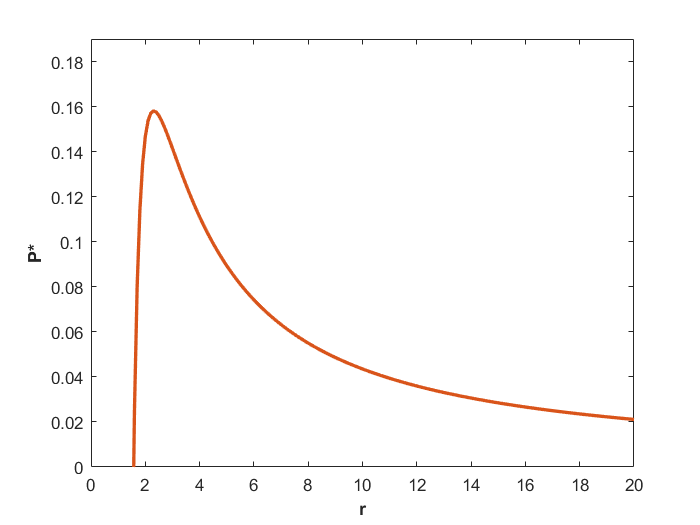
\includegraphics[width=\textwidth]{Images/FracBrayton_PvsR_B(a=1.85).png}
    \caption{Variasi \(\beta\), \(\alpha=1.85\).}
    \label{fig:FracBraytonPvsR_B}
  \end{subfigure}
  \caption{(a) \(P^*\) terhadap \(r\), divariasi terhadap \(\alpha\) dengan \(\beta\) konstan. (b) \(P^*\) terhadap \(r\), divariasi terhadap\(\beta\) dengan \(\alpha\) konstan.}
  \label{fig:FracBraytonPvsR}
\end{figure}
Pertama adalah \textit{power output} \(P^*\) terhadap parameter ekspansi \(r\). Secara umum, pola yang didapat sama, yaitu \(P^*\) meningkat secara tajam pada \(r\) rendah hingga titik sebuah titik stasioner. Setelah melewati titik tersebut, \(P^*\) akan perlahan menurun hingga konvergensi di \(P^* = 0\) pada \(r\rightarrow\infty\). Pada Gambar \ref{fig:FracBraytonPvsR_a} dapat dilihat pengaruh dari parameter fraksional \(\alpha\) terhadap \textit{power output}. Jelas bahwa penurunan nilai \(\alpha\) mengakibatkan penurunan nilai \(P^*\). Hal ini disebabkan pada nilai \(\alpha\) lebih rendah, partikel memiliki peluang yang cukup besar untuk mengambil jalur dengan aksi yang lebih tinggi. Aksi yang lebih tinggi inilah yang mengurangi keluaran daya dari siklus ini. Selain itu, meski tidak terlalu signifikan, namun \(\alpha\) juga menggeser titik di mana \(P^*\) mulai menjadi real positif. Pergeseran ini disebabkan oleh hubungan \(L_A\) dan \(L_B\) yang dapat berubah bergantung pada nilai \(\alpha\). Pada Gambar \ref{fig:FracBraytonPvsR_B} dapat dilihat bahwa meski dikatakan divariasi terhadap \(\beta\), parameter disipasi tidak memiliki pengaruh apa pun terhadap \textit{power output} dari siklus Brayton kuantum fraksional ini. 
\begin{figure}[H]
  \centering
  \begin{subfigure}{0.49\textwidth}
    \centering
    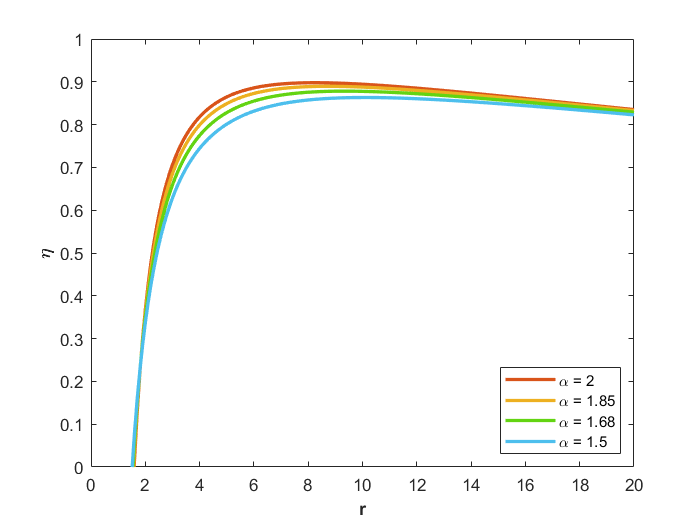
\includegraphics[width=\textwidth]{Images/FracBrayton_EtavsR_a(B=0.01).png}
    \caption{Variasi \(\alpha\), \(\beta=0.01\).}
    \label{fig:FracBraytonEtavsR_a}
  \end{subfigure}
  \hfill
  \begin{subfigure}{0.49\textwidth}
    \centering
    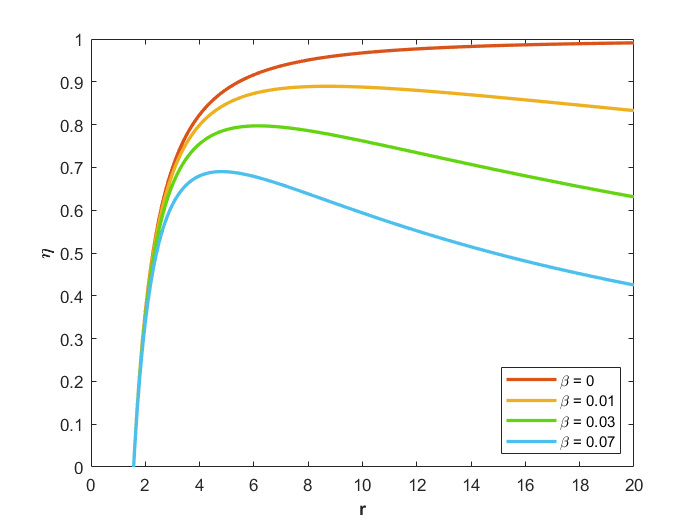
\includegraphics[width=\textwidth]{Images/FracBrayton_EtavsR_B(a=1.85).png}
    \caption{Variasi \(\beta\), \(\alpha=1.85\).}
    \label{fig:FracBraytonEtavsR_B}
  \end{subfigure}
  \caption{(a) \(\eta\) terhadap \(r\), divariasi terhadap \(\alpha\) dengan \(\beta\) konstan. (b) \(\eta\) terhadap \(r\), divariasi terhadap \(\beta\) dengan \(\alpha\) konstan.}
  \label{fig:FracBraytonEtavsR}
\end{figure}
Selanjutnya adalah efisiensi \(\eta\) terhadap \(r\). Nampak bahwa parameter \(\alpha\) dan \(\beta\) dapat mempengaruhi efisiensi siklus. Hanya saja, pengaruh parameter fraksional tidak terlalu signifikan terhadap efisiensi seperti yang dapat dilihat pada Gambar \ref{fig:FracBraytonEtavsR_a}. Selain itu, seperti yang terjadi pada \textit{power output}, \(\alpha\) juga sedikit menggeser titik di mana efisiensi mulai menjadi real positif. Secara umum, \(\alpha\) dapat mengurangi nilai efisiensi namun tidak begitu signifikan mengingat efisiensi lebih erat kaitannya dengan pertukaran panas daripada pergerakan partikel. Karenanya, pengaruh parameter disipasi tentu akan lebih signifikan terhadap efisiensi. Hal ini dibuktikan pada Gambar \ref{fig:FracBraytonEtavsR_B} di mana sedikit perubahan parameter disipasi mengakibatkan penurunan efisiensi secara signifikan. Bahkan, pada keadaan tanpa disipasi, meskipun nilai \(\alpha\) tidak 2, tetap dimungkinkan untuk siklus Brayton kuantum fraksional ini untuk mencapai nilai sempurna \(\eta=1\). Sedikit saja disipasi terjadi, maka hal tersebut tidak dimungkinkan lagi. 
\begin{figure}[H]
  \centering
  \begin{subfigure}{0.49\textwidth}
    \centering
    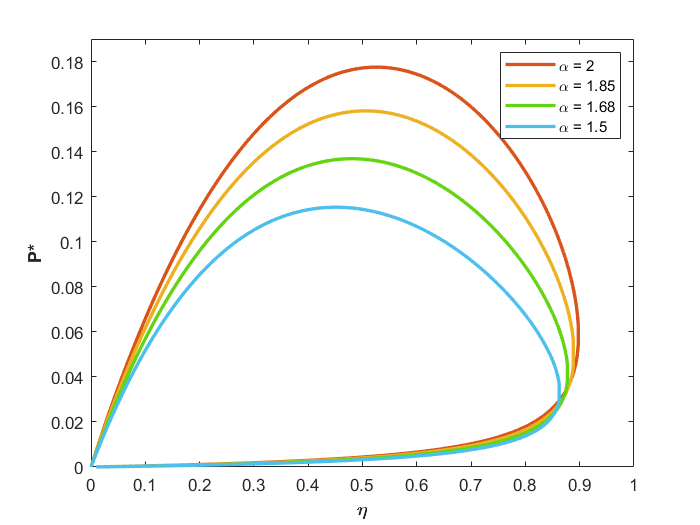
\includegraphics[width=\textwidth]{Images/FracBrayton_PvsEta_a(B=0.01).png}
    \caption{Variasi \(\alpha\), \(\beta=0.01\).}
    \label{fig:FracBraytonPvsEta_a}
  \end{subfigure}
  \hfill
  \begin{subfigure}{0.49\textwidth}
    \centering
    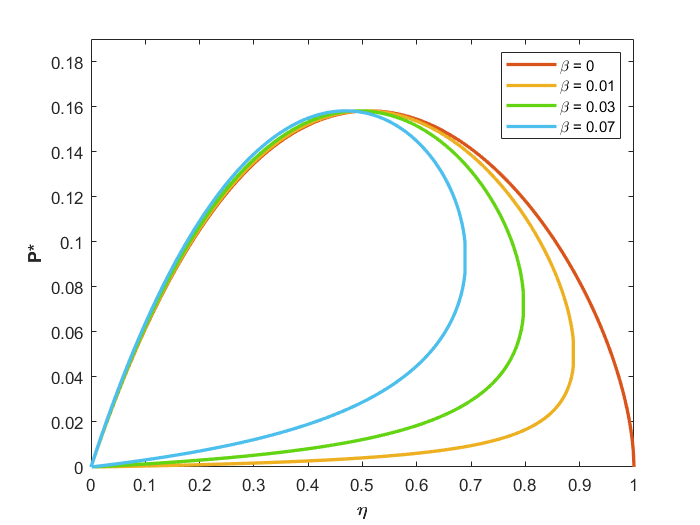
\includegraphics[width=\textwidth]{Images/FracBrayton_PvsEta_B(a=1.85).png}
    \caption{Variasi \(\beta\), \(\alpha=1.85\).}
    \label{fig:FracBraytonPvsEta_B}
  \end{subfigure}
  \caption{(a) \(P^*\) terhadap \(\eta\), divariasi terhadap \(\alpha\) dengan \(\beta\) konstan. (b) \(P^*\) terhadap \(\eta\), divariasi terhadap \(\beta\) dengan \(\alpha\) konstan.}
  \label{fig:FracBraytonPvsEta}
\end{figure}
Terakhir adalah \textit{power output} tak berdimensi \(P^*\) terhadap efisiensi \(\eta\). Pada Gambar \ref{fig:FracBraytonPvsEta_a}, keadaan yang dipilih adalah keadaan dengan disipasi sehingga tidak dimungkinkan untuk mencapai efisiensi 100\%. Di sini tampak jelas bahwa parameter fraksional \(\alpha\) mempengaruhi \(P^*\) lebih signifikan dibanding terhadap \(\eta\). Lalu, grafik ini juga menampilkan bahwa meski titik \(P^*\) dan \(\eta\) mulai menjadi real positif dapat bergeser oleh \(\alpha\), besar pergeserannya sama untuk \(P^*\) dan \(\eta\). Atau dapat dikatakan bahwa titik 0 dari \(P^*\) dan \(\eta\) untuk \(r\) kecil itu sama. Lalu Gambar \ref{fig:FracBraytonPvsEta_B} menampilkan \(P^*\) terhadap \(\eta\) dengan variasi pada parameter disipasi \(\beta\). Seperti yang sebelumnya telah disebutkan, \(\beta\) tidak mempengaruhi \(P^*\). Karena itulah titik puncak \(P^*\) tidak berubah. Hanya saja, nampak bahwa efisiensi berubah cukup signifikan akibat perubahan nilai \(\beta\). Hal ini mempertegas poin yang juga sudah dijelaskan sebelumnya di mana parameter disipasi mempengaruhi efisiensi tanpa memberi pengaruh pada \textit{power output}.

\section{Diskusi}
Dari hasil yang telah didapatkan, pengaruh parameter fraksional \(\alpha\) telah diketahui untuk semua siklus yang ditinjau. Didapati bahwa penurunan nilai \(\alpha\) akan menurunkan \textit{power output} serta efisiensi dari siklus mesin panas kuantum fraksional yang ditinjau. Pengaruh \(\alpha\) lebih signifikan terhadap parameter \textit{power output} dibanding terhadap efisiensi. Di sini, ketika nilai \(\alpha\) diturunkan, maka kerja yang dilakukan oleh siklus akan menurunan. Hal ini jelas terlihat dari persamaan-persamaan yang telah didapatkan sebelumnya. Meski demikian, signifikansi fisis dari parameter fraksional ini masih belum jelas. Untuk itu, perlu ditinjau representasi persamaan Schrodinger yang dilakukukan oleh Feynman. Representasi ini dikonstruksi dari aksi partikel yang memiliki definisi integral terhadap waktu dari Lagrangian seperti yang ditampilkan pada persamaan (\ref{eq:Action}). Namun, bentuk aksi juga dapat ditulis sebagai berikut \cite{Hilfer2000Applications}:
\begin{align}
    \mathcal{S} = \int p \dot{r} - \mathcal{H} \hspace{1px} dt \label{eq:Action2}
\end{align}
Dengan meninjau aksi dalam bentuk persamaan (\ref{eq:Action2}) serta Hamiltonian fraksional yang diberikan oleh persamaan (\ref{eq:FractionalHamiltonian}), dapat diketahui melalui deduksi yang cukup mudah bahwa,
\begin{align}
    \mathcal{S} \propto -D_\alpha |p|^\alpha \label{eq:Action3}
\end{align}
Bagian lengan kanan adalah komponen energi kinetik dari Hamiltonian fraksional. Dengan hubungan persamaan (\ref{eq:Action3}), jelas bahwa penurunan nilai \(\alpha\) akan cenderung berakibat pada peningkatan aksi. Hal ini mengindikasikan bahwa jalur yang diambil oleh partikel pada keadaan fraksional (\(1<\alpha<2\)) akan cenderung memiliki aksi yang lebih tinggi dibanding pada keadaan biasa (\(\alpha=2\)).
\par Kemudian adalah parameter disipasi \(\beta\). Dari hasil yang didapatkan, terlihat bahwa dimungkinkan untuk mendapatkan nilai efisiensi sempurna pada keadaan tanpa disipasi. Sekilas, hal ini tampak menyalahi hukum ke-2 termodinamika. Namun, jika ditinjau ulang hasil yang didapat, pada efisiensi 100\%, tidak ada \textit{power output} yang dihasilkan. Hal ini terjadi karena meskipun seluruh kalor diubah menjadi kerja, waktu siklus yang diperlukan untuk menyelesaikan satu siklus menjadi tak hingga. Oleh karena itu, tidak ada energi yang bisa diekstraksi sebagai \textit{power output} yang bermanfaat. Jika disipasi ditambahkan ke dalam sistem, terjadi penurunan efisiensi yang signifikan. Hal ini disebabkan oleh kenaikan faktor penyebut pada persamaan efisiensi akibat \(r\) yang jauh lebih cepat dibandingkan kenaikan faktor pembilangnya. Lalu jika nilai \(\beta\) dinaikkan, efisiensi akan smekin menurun secara signifikan karena kenaikan faktor penyebutnya akan semakin cepat seiring kenaikan \(r\) tanpa mengubah faktor pembilangnya. Meski demikian, parameter disipasi \(\beta\) ini tidak mempengaruhi \textit{power output} siklus sama sekali. Hal ini karena disipasi panas merupakan faktor tambahan pada panas yang masuk dan keluar dari siklus. Dalam definisi kerja, yang merupakan selisih antara kalor yang masuk dan keluar, faktor disipasi panas akan saling menghilangkan. Dengan kata lain, disipasi menambah kalor pada kedua sisi siklus secara seimbang sehingga tidak mengubah total \textit{power output}, tetapi secara signifikan menurunkan efisiensi.

\newpage















% \section{Sistem 1 Partikel}
% \par Pada bagian ini, persamaan energi terkuantisasi yang digunakan memiliki bentuk
% \begin{equation}
%     E_n = D_{\alpha}\left(\frac{\hbar\pi}{2L}\right)^{\alpha} n^{\alpha}
% \end{equation}
% Persamaan tersebut akan digunakan utuk perhitungan efisiensi dari ketiga mesin panas kuantum fraksional 1 partikel.

% \subsection{Siklus Carnot}
% Untuk mendapatkan efisiensi \((\eta)\) pada mesin Carnot, kuantitas yang dibutuhkan adalah \(Q_{AB}\) dan \(Q_{CD}\). Pertama, \(Q_{AB}\) dihitung di mana prosesnya isotermal atau isoenergetik pada konteks ini.
% \begin{align*}
%     dQ =& \Sigma_nE_ndP_n\\
%     dQ_{AB} =& E_1(L)dP_1(L) + E_2(L)dP_1(L)\\
%     =& (E_1(L)-E_2(L))dP_1(L)
% \end{align*}
% \(P_1(L)\) dan \(dP_1(L)\) diturunkan sebagai berikut:
% \begin{align*}
%     E_1(L_A) =& E_1(L)P_1(L) + E_2(L)P_2(L)\\
%     =& E_1(L)P_1(L) + E_2(L)(1 - P_1(L))\\
%     =& E_1(L)P_1(L) + E_2(L) - E_2(L)P_1(L))\\
%     E_1(L_A) - E_2(L) =& E_1(L)P_1(L) - E_2(L)P_1(L)\\
%     P_1(L) =& \frac{E_1(L_A) - E_2(L)}{E_1(L) - E_2(L)}\\
%     dP_1(L) =& \frac{d}{dL}\biggl(\frac{E_1(L_A) - E_2(L)}{E_1(L) - E_2(L)}\biggl)dL
% \end{align*}
% \(dP_1(L)\) disubstitusi kepada \(dQ_{AB}\) lalu diintegralkan sepanjang \(L_A\) ke \(L_B\) agar \(Q_{AB}\) bisa didapatkan
% \begin{align*}
%     Q_{AB} =& \int_{L_A}^{L_B}(E_1(L) - E_2(L))\frac{d}{dL}\biggl(\frac{E_1(L_A) - E_2(L)}{E_1(L) - E_2(L)}\biggl)dL\\
%     =& \int_{L_A}^{L_B} \biggl[D_{\alpha}\biggl(\frac{\hbar\pi}{2L}\biggl)^{\alpha} - D_{\alpha}\biggl(\frac{\hbar\pi}{2L}\biggl)^{\alpha}2^{\alpha}\biggl]\frac{d}{dL}\left[\frac{D_{\alpha}\left(\frac{\hbar\pi}{2L_A}\right)^{\alpha} - D_{\alpha}\left(\frac{\hbar\pi}{2L}\right)^{\alpha}2^{\alpha}}{D_{\alpha}\left(\frac{\hbar\pi}{2L}\right)^{\alpha} - D_{\alpha}\left(\frac{\hbar\pi}{2L}\right)^{\alpha}2^{\alpha}}\right] dL\\
%     =& D_{\alpha}\biggl(\frac{\hbar\pi}{2}\biggl)^{\alpha}\int_{L_A}^{L_B} \left[\frac{1}{L^{\alpha}} - \left(\frac{2}{L}\right)^{\alpha}\right] \frac{d}{dL}\left[\frac{\frac{1}{L_A^{\alpha}} - \left(\frac{2}{L}\right)^{\alpha}}{\frac{1}{L^{\alpha}} - \left(\frac{2}{L}\right)^{\alpha}}\right] dL\\
%     =& D_{\alpha}\biggl(\frac{\hbar\pi}{2}\biggl)^{\alpha}\int_{L_A}^{L_B} \frac{1 - 2^{\alpha}}{L^{\alpha}} \frac{\alpha L^{\alpha - 1}}{L_A^{\alpha}(1 - 2^{\alpha})} dL\\
%     =& \alpha D_{\alpha}\biggl(\frac{\hbar\pi}{2L_A}\biggl)^{\alpha} \int_{L_A}^{L_B} \frac{1}{L} dL\\
%     =& \alpha D_{\alpha}\biggl(\frac{\hbar\pi}{2L_A}\biggl)^{\alpha} \ln{\biggl(\frac{L_B}{L_A}\biggl)}
% \end{align*}
% Dikarenakan proses \(Q_{CD}\) dan \(Q_{AB}\) adalah proses yang serupa dengan arah yang berlawanan, maka \(Q_{CD}\) bisa didapatkan dengan menggunakan cara yang serupa
% \begin{align*}
%     Q_{CD} =& -\alpha D_{\alpha}\biggl(\frac{\hbar\pi}{2L_D}\biggl)^{\alpha} \ln{\biggl(\frac{L_C}{L_D}\biggl)}
% \end{align*}
% Kemudian, efisiensi bisa didapatkan menggunakan \(Q_{AB}\) dan \(Q_{CD}\)
% \begin{align*}
%     \eta =& 1 - \frac{\left|Q_{CD}\right|}{\left|Q_{AB}\right|}\\
%     =& 1 - \frac{\alpha D_{\alpha}\left(\frac{\hbar\pi}{2L_D}\right)^{\alpha} \ln{\left(\frac{L_C}{L_D}\right)}}{\alpha D_{\alpha}\left(\frac{\hbar\pi}{2L_A}\right)^{\alpha} \ln{\left(\frac{L_B}{L_A}\right)}}
% \end{align*}
% Untuk menyederhanakan persamaan, hubungan kesebandingan \(L_A \propto L_B\) dan \(L_C \propto L_D\) perlu dicari. Pertama, hubungan kesebandingan \(L_A \propto L_B\) dihitung sebagai berikut:
% \begin{align*}
%     E_1(L_A) =& E_2(L_B)\\
%     D_{\alpha}\left(\frac{\hbar\pi}{2L_A}\right)^{\alpha} =& D_{\alpha}\left(\frac{\hbar\pi}{2L_B}\right)^{\alpha}2^{\alpha}\\
%     L_B^{\alpha} =& 2^{\alpha}L_A^{\alpha}\\
%     L_B =& 2L_A
% \end{align*}
% Dengan menggunakan cara yang serupa, hubungan kesebandingan \(L_C \propto L_D\) bisa didapatkan
% \begin{align*}
%     L_C = 2L_D
% \end{align*}
% Yang mana bisa ditulis ulang sebagai berikut:
% \begin{align*}
%     \frac{L_B}{L_A} = \frac{L_C}{L_D} = 2
% \end{align*}
% Dengan begitu, bentuk paling sederhana dari persamaan efisiensi bisa didapatkan
% \begin{equation}
%     \eta = 1 - \left(\frac{L_A}{L_D}\right)^{\alpha}
% \end{equation}

% \subsection{Siklus Otto}
% Pada siklus Otto, kuantitas yang dibutuhkan untuk mendapatkan efisiensi \((\eta)\) adalah \(Q_{AB}\) dan \(Q_{CD}\). Pertama, \(Q_{AB}\) dihitung di mana prosesnya adalah isovolume atau \(L\) yang konstan dalam konteks ini.
% \begin{align*}
%     Q_{AB} =& \Delta U_{AB}\\
%     =& E_2(L_B) - E_1(L_A)\\
%     =& E_2(L_A) - E_1(L_A)\\
%     =& D_{\alpha}\left(\frac{\hbar\pi}{2L_A}\right)^{\alpha} 2^{\alpha} - D_{\alpha}\left(\frac{\hbar\pi}{2L_A}\right)^{\alpha}\\
%     =& D_{\alpha}\left(\frac{\hbar\pi}{2L_A}\right)^{\alpha}(2^{\alpha} - 1)
% \end{align*}
% Dengan menggunakan cara yang serupa, \(Q_{CD}\) bisa didapatkan
% \begin{align*}
%     Q_{AB} = - D_{\alpha}\left(\frac{\hbar\pi}{2L_D}\right)^{\alpha}(2^{\alpha} - 1)
% \end{align*}
% Dengan begitu, efisiensi mesin Otto bisa didapatkan
% \begin{align*}
%     \eta =& 1 - \frac{\left|Q_{CD}\right|}{\left|Q_{AB}\right|}\\
%     =& 1 - \frac{\alpha D_{\alpha}\left(\frac{\hbar\pi}{2L_D}\right)^{\alpha} (2^{\alpha} - 1)}{\alpha D_{\alpha}\left(\frac{\hbar\pi}{2L_A}\right)^{\alpha}(2^{\alpha} - 1)}
% \end{align*}
% Yang mana bisa disederhanakan menjadi
% \begin{equation}
%     \eta = 1 - \left(\frac{L_A}{L_D}\right)^{\alpha}
% \end{equation}

% \subsection{Siklus Brayton}
% Pada siklus ini, energi kuantisasi yang digunakan sama. Namun terdapat suatu besaran gaya (\(F\)) yang bekerja pada partikel yang perlu dihitung juga. \(F\) dinyatakan sebagai berikut:
% \begin{align*}
%     F =& - \frac{d}{dL}E_n\\
%     =& - \frac{d}{dL}D_{\alpha}\left(\frac{\hbar\pi}{2L}\right)^{\alpha} n^{\alpha}\\
%     =& \alpha D_{\alpha}\left(\frac{\hbar\pi}{2}\right)^{\alpha} \frac{n^{\alpha}}{L^{\alpha + 1}}
% \end{align*}
% Untuk mendapatkan efisiensi \(\eta\) pada siklus Brayton diperlukan kuantitas \(Q_{AB}\) dan \(Q_{CD}\). Pertama \(Q_{AB}\) dihitung di mana prosesnya adalah isobarik atau dalam konteks ini, \(F\) yang telah dinyatakan sebelumnya konstan selama proses berlangsung. Selain itu, untuk menghitung \(Q_{AB}\) dibutuhkan kuantitas lain yaitu \(W_{AB}\) dan \(U_{AB}\) yang harus dihitung secara terpisah. \(W_{AB}\) dihitung sebagai berikut:
% \begin{align*}
%     W_{AB} =& \int_{L_A}^{L_B}F(L)dL\\
%     =& F(L_A) \int_{L_A}^{L_B}dL\\
%     =& \alpha D_{\alpha}\left(\frac{\hbar\pi}{2}\right)^{\alpha} \frac{L_B - L_A}{L_A^{\alpha + 1}}
% \end{align*}
% Selanjutnya \(\Delta U_{AB}\) dihitung sebagai berikut:
% \begin{align*}
%     \Delta U_{AB} =& E_2(L_B) - E_1(L_A)\\
%     =& D_{\alpha}\left(\frac{\hbar\pi}{2L_B}\right)^{\alpha} 2^{\alpha} - D_{\alpha}\left(\frac{\hbar\pi}{2L_A}\right)^{\alpha}\\
%     =& D_{\alpha}\left(\frac{\hbar\pi}{2}\right)^{\alpha} \left(\frac{2^{\alpha}}{L_B^{\alpha}} - \frac{1}{L_A^{\alpha}}\right)
% \end{align*}
% Setelah itu, \(Q_{AB}\) didapatkan dengan menambahkan \(W_{AB}\) dan \(\Delta U_{AB}\)
% \begin{align*}
%     Q_{AB} =& W_{AB} + \Delta U_{AB}\\
%     =&\alpha D_{\alpha}\left(\frac{\hbar\pi}{2}\right)^{\alpha} \frac{L_B - L_A}{L_A^{\alpha + 1}} + D_{\alpha}\left(\frac{\hbar\pi}{2}\right)^{\alpha} \left(\frac{2^{\alpha}}{L_B^{\alpha}} - \frac{1}{L_A^{\alpha}}\right)\\
%     =& D_{\alpha}\left(\frac{\hbar\pi}{2}\right)^{\alpha} \left[\frac{\alpha (L_B - L_A)}{L_A^{\alpha + 1}} + \left(\frac{2^{\alpha}}{L_B^{\alpha}} - \frac{1}{L_A^{\alpha}}\right)\right]
% \end{align*}
% \(Q_{AB}\) dapat disederhanakan lebih lanjut dengan mencari hubungan antara \(L_A\) dan \(L_B\).
% \begin{align*}
%     F(L_A) =& F(L_B)\\
%     \alpha D_{\alpha}\left(\frac{\hbar\pi}{2}\right)^{\alpha} \frac{1}{L_A^{\alpha + 1}} =& \alpha D_{\alpha}\left(\frac{\hbar\pi}{2}\right)^{\alpha} \frac{2^{\alpha}}{L_B^{\alpha + 1}}\\
%     L_A^{\alpha + 1} =& \frac{L_B^{\alpha + 1}}{2^\alpha}\\
%     2^{\frac{\alpha}{\alpha + 1}}L_A =& L_B
% \end{align*}
% Sehingga \(Q_{AB}\) menjadi
% \begin{align*}
%     Q_{AB} =& D_{\alpha}\left(\frac{\hbar\pi}{2}\right)^{\alpha} \left[\frac{\alpha (2^{\frac{\alpha}{\alpha + 1}}L_A - L_A)}{L_A^{\alpha + 1}} + \left(\frac{2^{\alpha}}{(2^{\frac{\alpha}{\alpha + 1}}L_A)^{\alpha}} - \frac{1}{L_A^{\alpha}}\right)\right]\\
%     =& D_{\alpha}\left(\frac{\hbar\pi}{2}\right)^{\alpha} \left[\frac{\alpha (2^{\frac{\alpha}{\alpha + 1}} - 1)}{L_A^{\alpha}} + \frac{1}{L_A^\alpha}\left(\frac{2^{\alpha}}{2^{\frac{\alpha^2}{\alpha + 1}}} - 1\right)\right]\\
%     =& D_{\alpha}\left(\frac{\hbar\pi}{2L_A}\right)^{\alpha} \left[\alpha (2^{\frac{\alpha}{\alpha + 1}} - 1) + \left(\frac{2^{\alpha}}{2^{\frac{\alpha^2}{\alpha + 1}}} - 1\right)\right]
% \end{align*}
% Dengan metode serupa, \(Q_{CD}\) bisa didapat.
% \begin{align*}
%     Q_{CD} = - D_{\alpha}\left(\frac{\hbar\pi}{2L_D}\right)^{\alpha} \left[\alpha (2^{\frac{\alpha}{\alpha + 1}} - 1) + \left(\frac{2^{\alpha}}{2^{\frac{\alpha^2}{\alpha + 1}}} - 1\right)\right]
% \end{align*}
% Yang pada akhirnya, mengarah kepada didapatkannya efisiensi dari siklus Brayton.
% \begin{align*}
%     \eta =& 1 - \frac{\left|Q_{CD}\right|}{\left|Q_{AB}\right|}\\
%     =& 1 - \frac{D_{\alpha}\left(\frac{\hbar\pi}{2L_D}\right)^{\alpha} \left[\alpha (2^{\frac{\alpha}{\alpha + 1}} - 1) + \left(\frac{2^{\alpha}}{2^{\frac{\alpha^2}{\alpha + 1}}} - 1\right)\right]}{D_{\alpha}\left(\frac{\hbar\pi}{2L_A}\right)^{\alpha} \left[\alpha (2^{\frac{\alpha}{\alpha + 1}} - 1) + \left(\frac{2^{\alpha}}{2^{\frac{\alpha^2}{\alpha + 1}}} - 1\right)\right]}
% \end{align*}
% Setelah dilakukan penyederhanaan, persamaan menjadi
% \begin{equation}
%     \eta = 1 - \left(\frac{L_A}{L_D}\right)^\alpha
% \end{equation}

% \section{Sistem N Partikel}
% Karena jumlah partikel banyak, energi terkuantisasi yang digunakan memiliki bentuk yang sedikit berbeda dengan sebelumnya yaitu
% \begin{equation}
%     E_k = D_\alpha\left(\frac{\hbar\pi}{2L}\right)^\alpha\sum_{k=1}^Nk^\alpha
% \end{equation}
% Untuk keadaan dasar dan
% \begin{equation}
%     E_{M - N + k} = D_\alpha\left(\frac{\hbar\pi}{2L}\right)^\alpha\sum_{k=1}^N(M - N + k)^\alpha
% \end{equation}
% Untuk keadaan tereksitasi. Di mana \(M\) merupakan tingkat energi tertinggi dari sistem yang tereksitasi dan indeks \(k\) digunakan untuk membedakan penyebutannya dengan \(N\).

% \subsection{Siklus Carnot}
% Sama seperti sistem 1 partikel, untuk mendapatkan efisiensi diperlukan \(Q_{AB}\) dan \(Q_{CD}\). Namun akan terdapat beberapa permasalahan tambahan untuk menghitung efisiensi pada sistem banyak partikel. Untuk menghindari permasalahan tersebut dan menyederhanakan perhitungan, sistem dianggap sebagai sistem dengan 2 keadaan. Pada tiap partikelnya hanya dilihat keadaan awal dan akhirnya saja. Lalu untuk perhitungan \(Q_{AB}\), pertama ditinjau 1 partikel ke \(l\) yang berada dalam sistem. Energi terkuantisasi dari partikel tersebut adalah
% \begin{equation*}
%     E_l = D_\alpha\frac{\hbar\pi}{2L}l^\alpha
% \end{equation*}
% Karena sistem dianggap sebagai sistem 2 keadaan, maka probabilitas partikel tersebut selama proses \(A\) ke \(B\) dinyatakan sebagai berikut:
% \begin{equation*}
%     P_l(L) + P_{M-N+l}(L) = 1
% \end{equation*}
% Hal tersebut mirip seperti sistem 1 partikel yang telah diseselesaikan sebelumnya. Sehingga perhitungan panas yang melibatkan partikel ke \(l\) tersebut dapat dinyatakan secara langsung sebagai berikut:
% \begin{align*}
%     Q_l =& \int_{L_A}^{L_B} (E_l(L) - E_{M-N+l}(L)) \frac{d}{dL} \left(
%     \frac{E_l(L_A) - E_{M-N+l}(L)}{E_l(L) - E_{M-N+l}(L)} \right)dL\\
%     =& \int_{L_A}^{L_B} \left[ D_\alpha \left(\frac{\hbar\pi}{2L}\right)^\alpha l^\alpha -  D_\alpha \left(\frac{\hbar\pi}{2L}\right)^\alpha (M-N+l)^\alpha \right]\\
%     &\frac{d}{dL} \left[ \frac{D_\alpha \left(\frac{\hbar\pi}{2L}\right)^\alpha l^\alpha -  D_\alpha \left(\frac{\hbar\pi}{2L_A}\right)^\alpha (M-N+l)^\alpha}{D_\alpha \left(\frac{\hbar\pi}{2L}\right)^\alpha l^\alpha -  D_\alpha \left(\frac{\hbar\pi}{2L}\right)^\alpha (M-N+l)^\alpha} \right]dL\\
%     =& D_\alpha \left(\frac{\hbar\pi}{2}\right)^\alpha \int_{L_A}^{L_B} \left[\left( \frac{l}{L} \right)^\alpha - \left( \frac{M-N+l}{L} \right)^\alpha \right] \frac{d}{dL} \left[\frac{\left(\frac{lL}{L_A}\right)^\alpha - (M-N+l)^\alpha}{l^\alpha - (M-N+L)^\alpha} \right]dL\\
%     =& D_\alpha \left(\frac{\hbar\pi}{2}\right)^\alpha \int_{L_A}^{L_B} \frac{\alpha L^{\alpha-1}}{L^\alpha} \left(\frac{l}{L_A}\right)^\alpha dL\\
%     =& \alpha D_\alpha \left(\frac{\hbar\pi l}{2L_A}\right)^\alpha \int_{L_A}^{L_B} \frac{1}{L}dL\\
%     =& \alpha D_\alpha \left(\frac{\hbar\pi l}{2L_A}\right)^\alpha \ln{\left(\frac{L_B}{L_A}\right)}
% \end{align*}
% Selanjutnya, \(Q_{AB}\) didapat dengan menjumlahkan panas dari seluruh partikel yang terlibat selama proses.
% \begin{equation}
%     Q_{AB} = \alpha D_\alpha \left(\frac{\hbar\pi}{2L_A}\right)^\alpha \ln{\left(\frac{L_B}{L_A}\right)} \sum_{l=1}^N l^\alpha
% \end{equation}
% Lalu dengan menggunakan metode serupa, \(Q_{CD}\) bisa didapat.
% \begin{equation}
%     Q_{CD} = - \alpha D_\alpha \left(\frac{\hbar\pi}{2L_D}\right)^\alpha \ln{\left(\frac{L_C}{L_D}\right)} \sum_{l=1}^N l^\alpha
% \end{equation}
% Dengan begitu, efisiensi bisa didapatkan dan dapat dinyatakan sebagai berikut:
% \begin{align*}
%     \eta =& 1 - \frac{\left|Q_{CD}\right|}{\left|Q_{AB}\right|}\\
%     =& 1 - \frac{\alpha D_\alpha \left(\frac{\hbar\pi}{2L_D}\right)^\alpha \ln{\left(\frac{L_C}{L_D}\right)} \sum_{l=1}^N l^\alpha}{\alpha D_\alpha \left(\frac{\hbar\pi}{2L_A}\right)^\alpha \ln{\left(\frac{L_B}{L_A}\right)} \sum_{l=1}^N l^\alpha}\\
%     =& 1 - \frac{L_A^\alpha\ln{\left(\frac{L_C}{L_D}\right)}}{L_D^\alpha\ln{\left(\frac{L_B}{L_A}\right)}}
% \end{align*}
% Dengan menyatakan \(\frac{L_C}{L_D} = \frac{L_B}{L_A}\), bentuk paling sederhana dari efisiensi bisa didapat.
% \begin{equation}
%     \eta = 1 - \left(\frac{L_A}{L_D}\right)^\alpha
% \end{equation}
% Perubahan panjang yang dialami oleh semua partikel adalah sama. Sehingga, pernyataan yang digunakan untuk menyederhanakan bentuk efisiensi dapat dibuktikan dengan meninjau perubahan panjang yang dialami oleh 1 partikel. Untuk \(L_A\) dan \(L_B\) adalah sebagai berikut:
% \begin{align*}
%     E_l(L_A) =& E_{M-N+l}(L_B)\\
%     D_\alpha\left(\frac{\hbar\pi}{2L_A}\right)^\alpha l^\alpha =& D_\alpha\left(\frac{\hbar\pi}{2L_B}\right)^\alpha (M-N+l)^\alpha\\
%     \frac{L_B}{L_A} =& \frac{M-N+l}{l}
% \end{align*}
% Sedangkan untuk \(L_D\) dan \(L_C\) adalah sebagai berikut:
% \begin{align*}
%     E_l(L_D) =& E_{M-N+l}(L_C)\\
%     D_\alpha\left(\frac{\hbar\pi}{2L_D}\right)^\alpha l^\alpha =& D_\alpha\left(\frac{\hbar\pi}{2L_C}\right)^\alpha (M-N+l)^\alpha\\
%     \frac{L_C}{L_D} =& \frac{M-N+l}{l} = \frac{L_B}{L_A}
% \end{align*}

% \subsection{Siklus Otto}
% Serupa seperti siklus Carnot untuk N partikel, penyelesaian dilakukan dengan meninjau 1 partikel ke \(l\) yang ada pada sistem. Untuk mendapatkan efisiensi diperlukan \(Q_{AB}\) dan \(Q_{CD}\) yang dihitung sebagai berikut:
% \begin{align*}
%     Q_{l} =& \Delta U_l\\
%     =& D_\alpha\left(\frac{\hbar\pi}{2L_A}\right)^\alpha (M-N+l)^\alpha - D_\alpha\left(\frac{\hbar\pi}{2L_A}\right)^\alpha l^\alpha\\
%     =& D_\alpha\left(\frac{\hbar\pi}{2L_A}\right)^\alpha [(M-N+l)^\alpha - l^\alpha]\\
%     Q_{AB} =& D_\alpha\left(\frac{\hbar\pi}{2L_A}\right)^\alpha\sum_{l=1}^N[(M-N+l)^\alpha - l^\alpha]
% \end{align*}
% Dengan cara serupa didapatkan juga \(Q_{CD}\)
% \begin{align*}
%     Q_{CD} =& -D_\alpha\left(\frac{\hbar\pi}{2L_D}\right)^\alpha\sum_{l=1}^N[(M-N+l)^\alpha - l^\alpha]
% \end{align*}
% Dengan begitu efisiensi sistem bisa didapatkan,
% \begin{align*}
%     \eta =& 1 - \frac{\left|Q_{CD}\right|}{\left|Q_{AB}\right|}\\
%     =& 1 - \frac{D_\alpha\left(\frac{\hbar\pi}{2L_D}\right)^\alpha\sum_{l=1}^N[(M-N+l)^\alpha - l^\alpha]}{D_\alpha\left(\frac{\hbar\pi}{2L_A}\right)^\alpha\sum_{l=1}^N[(M-N+l)^\alpha - l^\alpha]}
% \end{align*}
% Yang mana dapat disederhanakan menjadi
% \begin{equation}
%     \eta = \left(\frac{L_A}{L_D}\right)^\alpha
% \end{equation}

% \subsection{Siklus Brayton}
% Sama seperti sebelumnya, \(Q_{AB}\) dan \(Q_CD\) diselesaikan dengan meninjau partikel ke \(l\) dalam sistem. Namun pada sistem ini terdapat kesulitan tambahan di mana \(Q\) dalam proses isobarik tidak dapat ditentukan secara langsung. Melainkan melalui nilai dari \(W\) dan \(\Delta U\). Panas yang dibawa oleh 1 partikel ke \(l\) dihitung sebagai berikut:
% \begin{align*}
%     W_l =& F(L_A)\int_{L_A}^{L_B}dL\\
%     =& \frac{\alpha D_\alpha}{L_A^{\alpha + 1}}\left(\frac{\hbar\pi l}{2}\right)^\alpha (L_B - L_A)\\
%     \Delta U_l =& E_{M-N+l}(L_B) - E_l(L_A)\\
%     =& D_\alpha\left(\frac{\hbar\pi}{2}\right)^\alpha\left[\frac{(M-N+l)^\alpha}{L_B^\alpha} - \frac{l^\alpha}{L_A^\alpha}\right]\\
%     Q_l =& D_\alpha\left(\frac{\hbar\pi}{2}\right)^\alpha\left[\frac{\alpha l^\alpha}{L_A^{\alpha+1}}(L_B - L_A) + \frac{(M-N+l)^\alpha}{L_B^\alpha} - \frac{l^\alpha}{L_A^\alpha}\right]
% \end{align*}
% Karena perubahan panjang \(L\) yang dialami oleh setiap partikel itu sama, maka hubungan antara \(L_A\) dan \(L_B\) dapat dicari dengan meninjau 1 partikel ke \(l\) saja. Hal ini juga dapat dilakukan terlebih dahulu sebelum semua partikel dijumlahkan. Hubungan \(L_A\) dan \(L_B\) didapat didapatkan sebagai berikut:
% \begin{align*}
%     F(L_A) =& F_(L_B)\\
%     \frac{\alpha D_\alpha}{L_A^{\alpha + 1}}\left(\frac{\hbar\pi l}{2}\right)^\alpha =& \frac{\alpha D_\alpha}{L_B^{\alpha + 1}}\left(\frac{\hbar\pi (M-N+l)}{2}\right)^\alpha\\
%     L_B^{\alpha + 1} =& \left(\frac{M-N+l}{l}\right)^\alpha L_A^{\alpha + 1}\\
%     L_B =& \left(\frac{M-N+l}{l}\right)^{\frac{\alpha}{\alpha + 1}}L_A
% \end{align*}
% Dengan begitu, \(Q_l\) didapat sebagai berikut:
% \begin{align*}
%     Q_l =& D_\alpha\left(\frac{\hbar\pi}{2}\right)^\alpha\left[\frac{\alpha l^\alpha}{L_A^{\alpha+1}}\left(\left(\frac{M-N+l}{l}\right)^{\frac{\alpha}{\alpha + 1}}L_A - L_A\right) + \frac{(M-N+l)^\alpha}{\left(\frac{M-N+l}{l}\right)^{\frac{\alpha^2}{\alpha + 1}}L_A^\alpha} - \frac{l^\alpha}{L_A^\alpha}\right]\\
%     =& D_\alpha\left(\frac{\hbar\pi}{2L_A}\right)^\alpha\left[\alpha l^\alpha\left(\left(\frac{M-N+l}{l}\right)^{\frac{\alpha}{\alpha + 1}} - 1\right) + \frac{(M-N+l)^\alpha}{\left(\frac{M-N+l}{l}\right)^{\frac{\alpha^2}{\alpha + 1}}} - l^\alpha\right]
% \end{align*}
% Sehingga, \(Q_{AB}\) dan \(Q_{CD}\) bisa didapat sebagai berikut:
% \begin{align*}
%     Q_{AB} =& D_\alpha\left(\frac{\hbar\pi}{2L_A}\right)^\alpha\sum_{l=1}^N \left[\alpha l^\alpha\left(\left(\frac{M-N+l}{l}\right)^{\frac{\alpha}{\alpha + 1}} - 1\right) + \frac{(M-N+l)^\alpha}{\left(\frac{M-N+l}{l}\right)^{\frac{\alpha^2}{\alpha + 1}}} - l^\alpha\right]\\
%     Q_{CD} =& -D_\alpha\left(\frac{\hbar\pi}{2L_D}\right)^\alpha\sum_{l=1}^N \left[\alpha l^\alpha\left(\left(\frac{M-N+l}{l}\right)^{\frac{\alpha}{\alpha + 1}} - 1\right) + \frac{(M-N+l)^\alpha}{\left(\frac{M-N+l}{l}\right)^{\frac{\alpha^2}{\alpha + 1}}} - l^\alpha\right]
% \end{align*}
% Dengan begitu efisiensi sistem bisa didapatkan,
% \begin{align*}
%     \eta =& 1 - \frac{\left|Q_{CD}\right|}{\left|Q_{AB}\right|}\\
%     =& 1 - \frac{D_\alpha\left(\frac{\hbar\pi}{2L_D}\right)^\alpha\sum_{l=1}^N \left[\alpha l^\alpha\left(\left(\frac{M-N+l}{l}\right)^{\frac{\alpha}{\alpha + 1}} - 1\right) + \frac{(M-N+l)^\alpha}{\left(\frac{M-N+l}{l}\right)^{\frac{\alpha^2}{\alpha + 1}}} - l^\alpha\right]}{D_\alpha\left(\frac{\hbar\pi}{2L_A}\right)^\alpha\sum_{l=1}^N \left[\alpha l^\alpha\left(\left(\frac{M-N+l}{l}\right)^{\frac{\alpha}{\alpha + 1}} - 1\right) + \frac{(M-N+l)^\alpha}{\left(\frac{M-N+l}{l}\right)^{\frac{\alpha^2}{\alpha + 1}}} - l^\alpha\right]}
% \end{align*}
% Yang mana juga dapat disederhanakan menjadi
% \begin{equation}
%     \eta = \left(\frac{L_A}{L_D}\right)^\alpha
% \end{equation}
